% Copyright (c) 2014,2016,2018 Casper Ti. Vector
% Public domain.

\chapter{\emph{decryst} 的使用方法和常用技巧}\label{chap:decr-usage}

本章将以 AMCSD 数据库\parencite{downs2003}中若干个不同晶系和复杂度的结构为例,
循序渐进地演示 \emph{decryst} 的基本用法和常用技巧;目前 \emph{decryst} 中自带了
\ce{Al2O3}(AMCSD 代号:0009325)、\ce{As2S3}(0010733)、\ce{PbSO4}(0005558)
和“0009563”等 4 个结构作为示例。此外,因为有一位用户在 \emph{decryst} 的试用阶段
建议再增加几个不同晶系和复杂度的示例,本人在 AMCSD 中搜索 $a$、$b$、$c$ 均介于
\SIrange{8}{16}{\angstrom} 的结构,在第一页结果中去除过于简单或过于复杂的
结构后选取了 “0000158”“0000219”“0000220”“0000428”“0000589” 等 5 个结构。
各代号所对应的化学式见相应小节;在本章的演示中,以上所有
结构在求解时均忽略 H 原子\footnote{%
	有必要指出,在结构精修中利用 X 射线衍射数据处理 H 原子是可行且
	有很强实际意义的,相关研究可参考文献\parencite{cooper2010}。%
},所有时间测量均在 Intel i7-3720QM CPU 上进行。

\section{\emph{decryst} 的基本用法}

在本节中,第 \ref{ssec:decr-fmt} 小节将介绍 \emph{decryst} 中主控程序(参考第
\ref{ssec:decr-arch} 小节)的输入格式,第 \ref{ssec:decr-base} 小节将演示
主控程序的用法,以及用 \emph{decryst} 进行结构测定的基本流程。在此基础之上,
第 \ref{ssec:decr-auto} 小节将讨论对全局最优化步骤中得到的评价指标相近的解进行
手工(目视)筛选的技术,并演示结合自动化工具使用 \emph{decryst} 的基本方法。第
\ref{ssec:epc-rank} 小节将初步演示和讨论对等效点系组合(EPC)进行筛选的方法。

\subsection{\emph{decryst} 中主控程序的输入格式}\label{ssec:decr-fmt}

如第 \ref{ssec:decr-arch} 小节所述,\emph{decryst} 中面向用户的核心接口由
主控程序 \verb|decr_utils| 提供。因此为了使用 \emph{decryst} 进行结构测定,
我们最先须要编写的是 \verb|decr_utils| 的输入文件(称为 \myterm{decr 文件},
详细格式参考 \verb|doc/usage/format.txt|)。首先以
\ce{Al2O3} 结构为例,其 decr 文件如下所示\footnote{%
	AMCSD 中的衍射数据不含半高宽(FWHM)字段,
	因此本章所有 decr 文件中 FWHM 值均为粗略的估计值。%
}:
\begin{Verbatim}
\cm{# (Lines beginning with `#' are comments and are ignored.)}
\cm{# ID of space group, (a, b, c), (alpha, beta, gamma).}
167a	4.7602 4.7602 12.9933	90 90 120
\cm{# Combination factor `mu', and some other control parameters.}
0.25 0.75 0.875	0.5 1.0
\cm{# Global EPC constraints (`--' for the defaults).}
--

\cm{# Atom species, number of atoms, EPC constraints, already}
\cm{# guessed EPCs with unknown coordinates (`--' for none).}
Al3+	12	--	--
O2-	18	--	--
\cm{# Pairwise zoom factors.}
1.6:0-0
\cm{# Wyckoff positions and coordinates for already solved atoms.}
\cm{#0@c1}	\cm{0}	\cm{0}	\cm{0.14784}

\cm{# Data for individual reflections:}
\cm{# 2-theta, FWHM, hkl, multiplicity, intensity.}
25.59	0.2	0 1 2	6	61.91
35.17	0.2	1 0 4	6	96.62
\cm{# (... further data lines left out for brevity ...)}

\end{Verbatim}

其中指定各 $hkl$ 所对应衍射数据的那些行以及指定空间群和晶胞参数的一行意义应该
很明显,唯一需要注意的是空间群的代号须要根据 \verb|wyck.json| 进行设定,例如
上述示例中 \verb|167a| 表示采用 $R\bar3c$ 空间群的六方表示。晶胞参数之后的一行
数据指定结构测定中使用的一些参数(详见 \verb|format.txt|),
其中最重要的是第 1 个和第 4 个:前者是组合因子 $\mu$(参考第
\ref{ssec:eval-func} 小节),而后者是 Lorentz{--}极化因子公式\footnote{%
	这一公式和国际晶体学表\parencite[620]{prince2004}中的公式是兼容的:
	事实上,对前者而言的 $p$ 正是对后者而言的 $A / (1 + A)$。%
}中的参数 $p$:
\begin{equation}
	LP = \frac{(1 - p) + p\cos^2 2\theta}{\sin2\theta \sin\theta}\mcstop
\end{equation}
$\mu$ 等参数之后的一行数据指定对晶胞中总 EPC 的额外约束(参考第
\ref{ssec:incr-epc} 小节),其写法形如 \verb|0-3 1-2|,其中每个字段对应于一个
Wyckoff 位置($a$、$b$、$\cdots$,其顺序根据 \verb|wyck.json| 中指定空间群
Wyckoff 位置的列表确定)总占据数的下限和上限。下限和上限都可省略,表示不对相应值
设定额外约束;此外,\verb|decr_utils| 会自动设定所有固定 Wyckoff 位置的占据数
上限不超过 1。最后,如果所有 Wyckoff 位置的总占据数均无额外约束,那么设定这一
约束的行可以被简写为“\verb|--|”,正如上述 \ce{Al2O3} 的例子所示。

晶胞化学式和对单元素 EPC 的约束由形如
\begin{Verbatim}
Al3+	12	--	--
\end{Verbatim}
的数据行指定。其中第 1 个字段是元素的代号,其半径\footnote{%
	中性原子采用共价半径\parencite{cordero2008},
	而离子采用离子半径\parencite{shannon1976}。%
}和散射因子数据分别会从 \verb|rad.json| 和 \verb|asf.json| 中读取;两者
所需元素代号不同时可使用形如 \verb|S6+;S| 的写法,而“混合元素”可用形如
\verb|0.6Fe2+,0.3Fe3+| 的写法来指定。第 2 个字段是晶胞中相应元素的
总原子数。第 3、4 个字段分别指定相应元素占据数的下限和上限,
写法形如 \verb|a2b1|(注意这和第 \ref{ssec:incr-epc} 小节中所用
EPC 表达式的相似性);其中未写出的 Wyckoff 位置均视作未设定额外约束,
而所有 Wyckoff 位置均无额外约束时相应字段可写为“\verb|--|”。

对缩放因子(参考第 \ref{ssec:cryst-sap} 小节,默认为 1)由形如
\begin{Verbatim}
1.1:0,1-1,2	1.2:2-2
\end{Verbatim}
的数据行\footnote{%
	即输入文件中除了空行和(以“\texttt{\#}”开头的)注释行之外的那些行。%
}指定,其中每个字段中“\verb|:|”之前为缩放因子的值,之后为被赋予相应
缩放因子的原子对:\verb|0,1-0,1| 会被展开为 \verb|0-0|、\verb|0-1| 和
\verb|1-1|。这里元素的编号根据晶胞化学式部分各元素被定义的顺序而定,
从零开始计数:例如在上述的 \ce{Al2O3} 示例中,\verb|0-0| 表示的是
\ce{Al^{3+}}--\ce{Al^{3+}} 原子对。已知位置的独立原子\footnote{%
	只有部分坐标已知的独立原子也可以用这种数据行表示,
	详见 \texttt{format.txt}。%
}由形如
\begin{Verbatim}
0@c1	0	0	0.14784
\end{Verbatim}
的数据行指定。在上述的 \ce{Al2O3} 示例中,以上数据行表示第 1 种元素(编号为 0,
即 \ce{Al^{3+}})占据 1 组 $c$ 位置,其中一个原子的坐标为 $(0, 0, 0.14784)$。

关于 \emph{decryst} 所用各类输入文件的格式,最后须要指出一些小但值得注意的技术
细节。首先,所有输入文件都只支持 Unix 中常用的 LF(\verb|\n|)换行符,而不支持
Windows 中常用的 CRLF(\verb|\r\n|)换行符,因此用户在 Windows 上编写的输入文件
一般须要经过 \verb|dos2unix| 等工具的转换。其次,输入文件中的空行(包括文件
末尾的空行,例如上述 \ce{Al2O3} 示例中的最后一行)具有特殊作用,不可随意添加或
删除。最后,数据行中空白字符(空格和制表符 \verb|\t|)可以混合使用,但建议
在不同类型的行中有规律地使用空白字符,从而方便利用文本处理工具进行自动化的
修改(参考第 \ref{ssec:heavy-atom} 和 \ref{ssec:epc-filter} 小节)。

\subsection{基本求解流程:以 \ce{Al2O3} 和 \ce{As2S3} 为例}\label{ssec:decr-base}

如第 \ref{ssec:decr-para} 小节所述,\emph{decryst} 将结构测定划分为生成
EPC 列表、对各 EPC 进行统计分析、对每个 EPC 进行全局最优化和导出解模型等
4 个主要步骤。这里先继续以 \ce{Al2O3} 的结构测定为例;在编写完 decr
文件之后,用以下命令即可生成 EPC 列表:
\begin{Verbatim}
\cm{$} decr_utils comb /path/to/Al2O3.txt | tee combs.list
\end{Verbatim}
其输出(称为 \myterm{combs 文件},详见 \verb|format.txt|)应如下所示:
\begin{Verbatim}
\cm{>} 0@a1b1,1@d1.cr	0@a1b1,1@d1
\cm{>} 0@a1b1,1@e1.cr	0@a1b1,1@e1
\cm{>} ...
\end{Verbatim}
其中两个字段分别为该 EPC 所对应的文件名和表达式。有必要特别提请注意的是,combs
文件中的 EPC 只考虑未分配到任何 Wyckoff 位置的原子,而且 decr 文件中已知 Wyckoff
位置的两种原子是被分开计数的:例如要是 decr 文件中指定了某元素的占据数上限
约束为 \verb|c3|、下限约束为 \verb|c1|,且该元素还有一个坐标已知的 \verb|c1|
占据,那么该元素在 combs 文件列出的 EPC 中最多会占据 1 组 $c$ 位置。此外,如果
所有原子均已在 decr 文件中分配到确定的 Wyckoff 位置,那么在此条件下只可能生成一个
“空的”EPC,而该 EPC 会被显示为 \verb|nil|。有了 combs 文件,我们就可以
实际生成各 EPC 所对应的用于 \emph{decryst} 中底层程序的输入文件\footnote{%
	这里的 EPC 文件名和下文中各 EPC 的全局最优化参数都是可以修改的;
	分两步生成 cryst 文件是为了在分步求解复杂结构时(例如在使用重原子法时,
	参考第 \ref{sec:decr-adv} 节)方便管理各步骤所需的输入文件。%
}(称为 \myterm{cryst 文件}\footnote{%
	本文中的各个示例不涉及其格式,因此本文不对其进行讨论,
	但其细节可参考 \texttt{format.txt};其余未注明
	“详见 \texttt{format.txt}”等字样的输入文件也类似。%
}):
\begin{Verbatim}
\cm{$} decr_utils dump /path/to/Al2O3.txt < combs.list | tee crysts.list
\end{Verbatim}
其输出(称为 \myterm{crysts 文件},详见 \verb|format.txt|)应如下所示:
\begin{Verbatim}
\cm{>} 0 0 - - - - -	0@a1b1,1@d1.cr
\cm{>} 1 1000 100 0.01 - - -	0@a1b1,1@e1.cr
\cm{>} ...
\end{Verbatim}
在 crysts 文件中,最后一个字段是 cryst 文件的文件名(可以注意到相应的文件已在
当前目录生成),第一个字段是相应 EPC 的维数;第 2--4 个字段分别为统计分析中的
样本数和 Lam 算法(参考第 \ref{ssec:decr-para} 小节)中的
$\tau$、$\lambda$ 参数\footnote{%
	其中零维 EPC 的样本数显示为 0(实际为 1)是出于方便自动化
	的考虑;这些 EPC 的 $\tau$ 和 $\lambda$ 显示为“\texttt{-}”,
	表示这两个参数无意义,因为这些 EPC 不需要全局最优化。%
}(后者取更小的值时,最优化会更精细但更耗时);第 5--7 个字段分别为相应
EPC 所产生晶体模型目标函数值 $E$ 的平均值、标准差和已知最佳值
(目前均显示为“\texttt{-}”,表示这些参数的值未知)。

\emph{decryst} 在对 EPC 进行统计分析和全局最优化时支持并行和分布式计算,而相应的
设定是通过 \myterm{hosts 文件}进行的,其详细格式参考 \verb|format.txt| 及其同一
目录中的 \verb|cmdline.txt|。\verb|doc/example/hosts.conf| 是 \emph{decryst}
自带的一个和 \verb|doc/scripts| 目录中脚本兼容的示例 hosts 文件,用户可根据自身
需求对其进行修改。此外,为了能正确调用包装脚本(参考第 \ref{ssec:decr-arch}
小节),\verb|scripts| 目录须要在搜索路径 \verb|$PATH| 中,而且
\verb|decr_mcs|、\verb|decr_lsa| 和 \verb|decr_sas| 须要安装到所有远程机器上。
在正确进行以上配置之后,我们便可以对上一步生成的 cryst 文件进行统计分析:
\begin{Verbatim}
\cm{$} decr_utils stat stat.sh /path/to/hosts.conf < crysts.list |
  tee crysts.stat
\end{Verbatim}
其输出应大致如下:
\begin{Verbatim}
\cm{>} 0 0 - - - - 0.385611	0@a1b1,1@d1.cr
\cm{>} 2 1000 200 0.01 0.530822 0.165276 0.045932	0@c1,1@e1.cr
\cm{>} ...
\end{Verbatim}
可见平均值、标准差、最佳值已被实际值取代;对于零维 EPC,只有最佳值有意义,
因此平均值和标准差仍显示为“\texttt{-}”。在获得统计分析的结果之后,
我们便可以进行全局最优化:
\begin{Verbatim}
\cm{$} decr_utils optim optim.sh /path/to/hosts.conf < crysts.stat |
  tee crysts.optim | sort -k7g
\end{Verbatim}
其输出应大致如下:
\begin{Verbatim}
\cm{>} 2 1000 200 0.01 0.530822 0.165276 0.0298237	0@c1,1@e1.cr
\cm{>} 1 1000 100 0.01 0.473024 0.157376 0.209828	0@a1b1,1@e1.cr
\cm{>} ...
\end{Verbatim}
注意其中最佳值已被替换为全局最优化步骤所得解模型的相应值,以及当前目录中生成了
用于记录全局最优化过程的 \verb|.log| 文件(称为 \myterm{crlog 文件}),如
\verb|0@c1,1@e1.log|。此外因为零维 EPC 不需要全局最优化,所以 crysts 文件中的
相应行会被 \verb|decr_utils| 的 \verb|optim| 子命令原样输出。

如上述输出(已用 \verb|sort| 命令排序)所示,\verb|0@c1,1@e1| 是 \ce{Al2O3}
唯一可行的 EPC。最后,我们可以将全局最优化的结果和原 decr 文件合并,
以产生各解模型所对应的 decr 文件和 CIF 文件:
\begin{Verbatim}
\cm{$} decr_utils merge /path/to/Al2O3.txt < combs.list
\end{Verbatim}
其输出应如下所示:
\begin{Verbatim}
\cm{>} 0@a1b1,1@d1.cr
\cm{>} 0@a1b1,1@e1.cr
\cm{>} ...
\end{Verbatim}
正确解所对应的 decr 文件和 CIF 文件分别是 \verb|0@c1,1@e1.txt|
和 \verb|0@c1,1@e1.cif|,后者可以直接在可视化软件中查看。
以上求解过程(除去人工步骤之后)耗时不到 \SI{1}{\second}。

\ce{As2S3}($P2_1/c$)的 decr 文件如下所示(注意其中因为缺少 \ce{As^{3+}}、%
\ce{S^{2-}} 的原子散射因子数据而采用了电中性 As、S 原子的数据,
参考第 \ref{ssec:decr-fmt} 小节):
\begin{Verbatim}
\cm{# sg, abc, angles; ctl, extra; limits.}
14a	4.256 9.577 12.191	90 109.75 90
0.25 0.75 0.875	0.5 1.0
--

\cm{# rad/asf, n, limits, comb.}
As3+;As	8	--	--
S2-;S	12	--	--

\cm{# 2theta, fwhm, hkl, mult, val.}
12.04	0.1	0 1 -1	4	12.34
18.02	0.1	0 1 -2	4	15.82
\cm{# (... further lines omitted ...)}
\end{Verbatim}
仿照以上步骤,其结构可以用完全类似的方法进行求解,除去人工步骤之后耗时约
\SI{15}{\second}。在求解的过程中,可以注意到正确 EPC \verb|0@e2,1@e3| 耗时远多于
其它所有 EPC,因为其维数(15)明显高于其它 EPC(均不超过 12);此外,\ce{As2S3}
有时一次全局最优化不能得到正确的解模型,需要多次求解。对于这类 EPC,并行的
全局最优化可以用于缩短单个 EPC 求解所需的时间,例如对 \ce{As2S3}
的 \verb|0@e2,1@e3| EPC 可以使用以下命令:
\begin{Verbatim}
\cm{$} grep 0@e2,1@e3 < crysts.list |
  decr_utils poptim server.sh hosts.conf | tee 0@e2,1@e3.log
\end{Verbatim}
需要注意的是 \verb|decr_utils| 的 \verb|poptim| 子命令只接受单行的 crysts 文件,
而且输出的是 crlog 文件而非 crysts 文件,因此用户须要自行管理其输出。

\subsection{实际求解:以“0000220”和“0000589”结构为例}\label{ssec:decr-auto}

“0000220”结构($Ia\bar3d$)的 decr 文件如下所示(注意其中一价原子被表示为
\verb|Li1+|、\verb|Na1+| 和 \verb|F1-|,这和 \verb|wyck.json| 是一致的,
参考第 \ref{ssec:decr-fmt} 小节):
\begin{Verbatim}
\cm{# sg, abc, angles; ctl, extra; limits.}
230	12.122 12.122 12.122	90 90 90
0.25 0.75 0.875	0.5 1.0
--

\cm{# rad/asf, n, limits, comb.}
Li1+	24	--	--
Na1+	24	--	--
Al3+	16	--	--
F1-	96	--	--
\cm{# zooms.}
1.4:2-2

\cm{# 2theta, fwhm, hkl, mult, val.}
17.92	0.2	2 1 1	24	11.87
20.73	0.2	2 2 0	12	100.00
\cm{# (... further lines omitted ...)}
\end{Verbatim}
该结构可以使用第 \ref{ssec:decr-base} 小节中的方式求解:其总 EPC 数为 28,单个
EPC 维数为 2--3,除去人工步骤之后求解总耗时约 \SI{5}{s},可直接得到目标函数值
$E = 0.0278$ 的正确解;正确 EPC 为 \verb|0@d1,1@c1,2@a1,3@h1|,
而其余 EPC 所得解的 $E$ 值至少为 0.11。

“0000589”结构($Pm\bar3m$)的 decr 文件如下所示:
\begin{Verbatim}
\cm{# sg, abc, angles; ctl, extra; limits.}
221	10.358 10.358 10.358	90 90 90
0.25 0.75 0.875	0.5 1.0
--

\cm{# rad/asf, n, limits, comb.}
Li1+	1	--	--
K1+	6	--	--
Fe2+	24	--	--
S2-;S	26	--	--
Cl1-	1	--	--

\cm{# 2theta, fwhm, hkl, mult, val.}
8.54	0.2	1 0 0	6	56.41
12.08	0.2	1 1 0	12	38.10
\cm{# (... further lines omitted ...)}
\end{Verbatim}
该结构的总 EPC 数为 2416,单个 EPC 维数为 5--9。其依然可以
按照上述各结构的方式求解,所得结果通常大致如下\footnote{%
	因为所使用算法中随机因素的缘故,实际结果中 $E \approx 0.075$ 的 EPC 数可能
	发生一定程度的浮动;在使用 \emph{decryst} 默认的参数时,其一般为 1--2。%
}:
\begin{Verbatim}
\cm{>} [...] 0.677702 0.0638962 0.0456528	0@b1,1@f1,2@m1,3@e1g1h1,4@a1.cr
\cm{>} [...] 0.676874 0.0680791 0.0469421	0@b1,1@e1,2@m1,3@f1g1h1,4@a1.cr
\cm{>} [...] 0.682297 0.0653026 0.0740492	0@a1,1@e1,2@m1,3@f1g1h1,4@b1.cr
\cm{>} [...] 0.686445 0.060813 0.0749921	0@a1,1@f1,2@m1,3@e1g1h1,4@b1.cr
\cm{>} [...] 0.697594 0.0678327 0.133365	0@a1,1@f1,2@m1,3@e1g1j1,4@b1.cr
\cm{>} ...
\end{Verbatim}
从 $E$ 值可见只有前 4 个 EPC 可能是合理的,又由 $(1/2, 1/2, 1/2)$ 平移使
$Pm\bar3m$ 空间群中 $a/b$、$c/d$、$e/f$、$i/j$、$k/l$ 位置互变并保持其它
Wyckoff 记号不变可知这 4 个 EPC 是两对等价 EPC。在可视化软件中查看这两对
EPC 生成的解,可见在 \verb|0@b1,1@f1,...| 和 \verb|0@a1,1@e1,...|
的解中 \ce{Cl-} 均被 \ce{S^{2-}} 配位(图 \ref{fig:589-sol}(c,d)),
这显然是错误的。在 \verb|0@b1,1@e1,...|(图 \ref{fig:589-sol}(a))和
\verb|0@a1,1@f1,...|(图 \ref{fig:589-sol}(b))的解中,即使不考虑后者
\ce{K+}--\ce{Fe^{2+}} 键长过短的问题,只根据 $E$ 值也可以知道前者是
唯一合理的解。除去人工步骤之后,“0000589”求解总耗时约 \SI{5}{\minute}。

\begin{figure}[htbp!]\bfcmd
\ffigbox{\begin{subfloatrow}
	\setlength{\columnsep}{1.5em}
	\ffigbox[0.32\textwidth]%
		{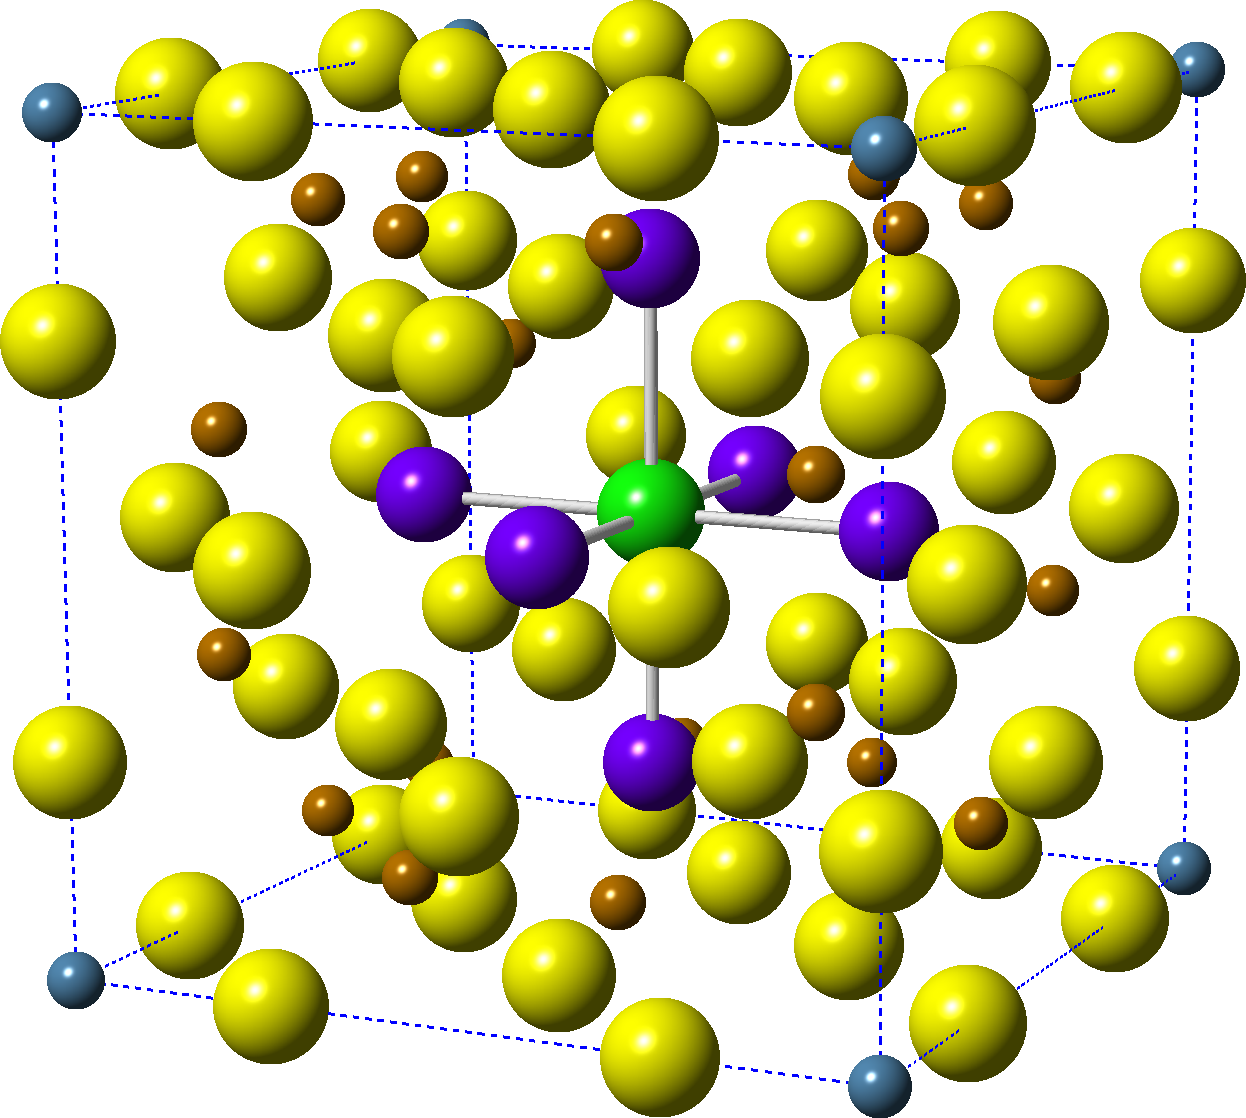
\includegraphics[height = 0.25\textwidth]{img/589-sol-1}}%
		{\caption{\texttt{0@a1,1@f1}($E = 0.0469$)}}
	\ffigbox[0.32\textwidth]%
		{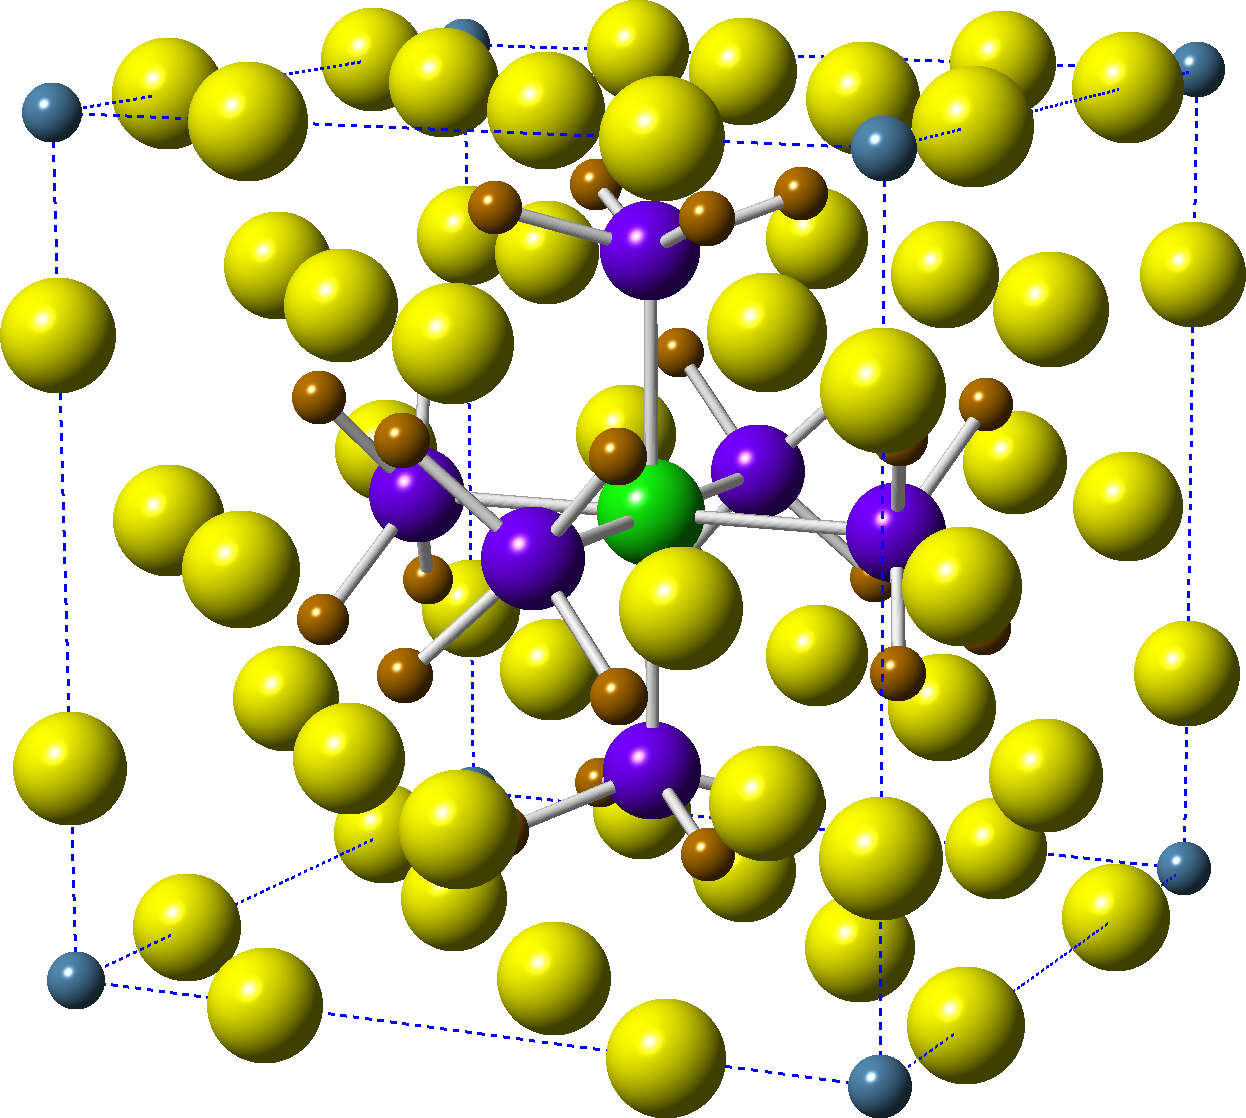
\includegraphics[height = 0.25\textwidth]{img/589-sol-2}}%
		{\caption{\texttt{0@a1,1@f1}($E = 0.0740$)}}
\end{subfloatrow}\\[0.5em]\begin{subfloatrow}
	\setlength{\columnsep}{1.5em}
	\ffigbox[0.32\textwidth]%
		{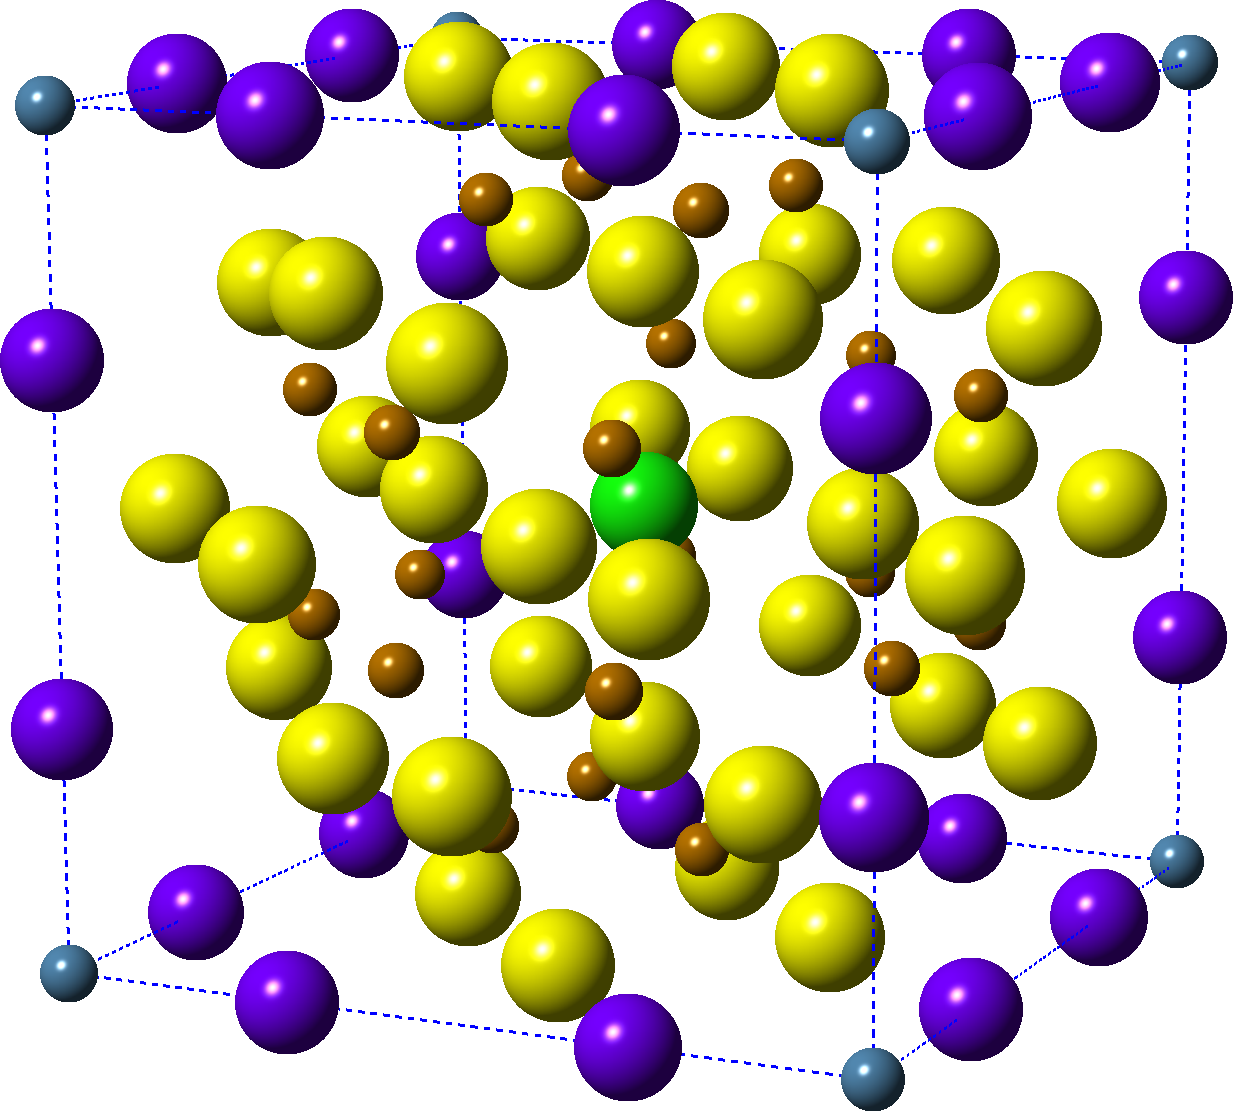
\includegraphics[height = 0.25\textwidth]{img/589-sol-3}}%
		{\caption{\texttt{0@a1,1@e1}($E = 0.0457$)}}
	\ffigbox[0.32\textwidth]%
		{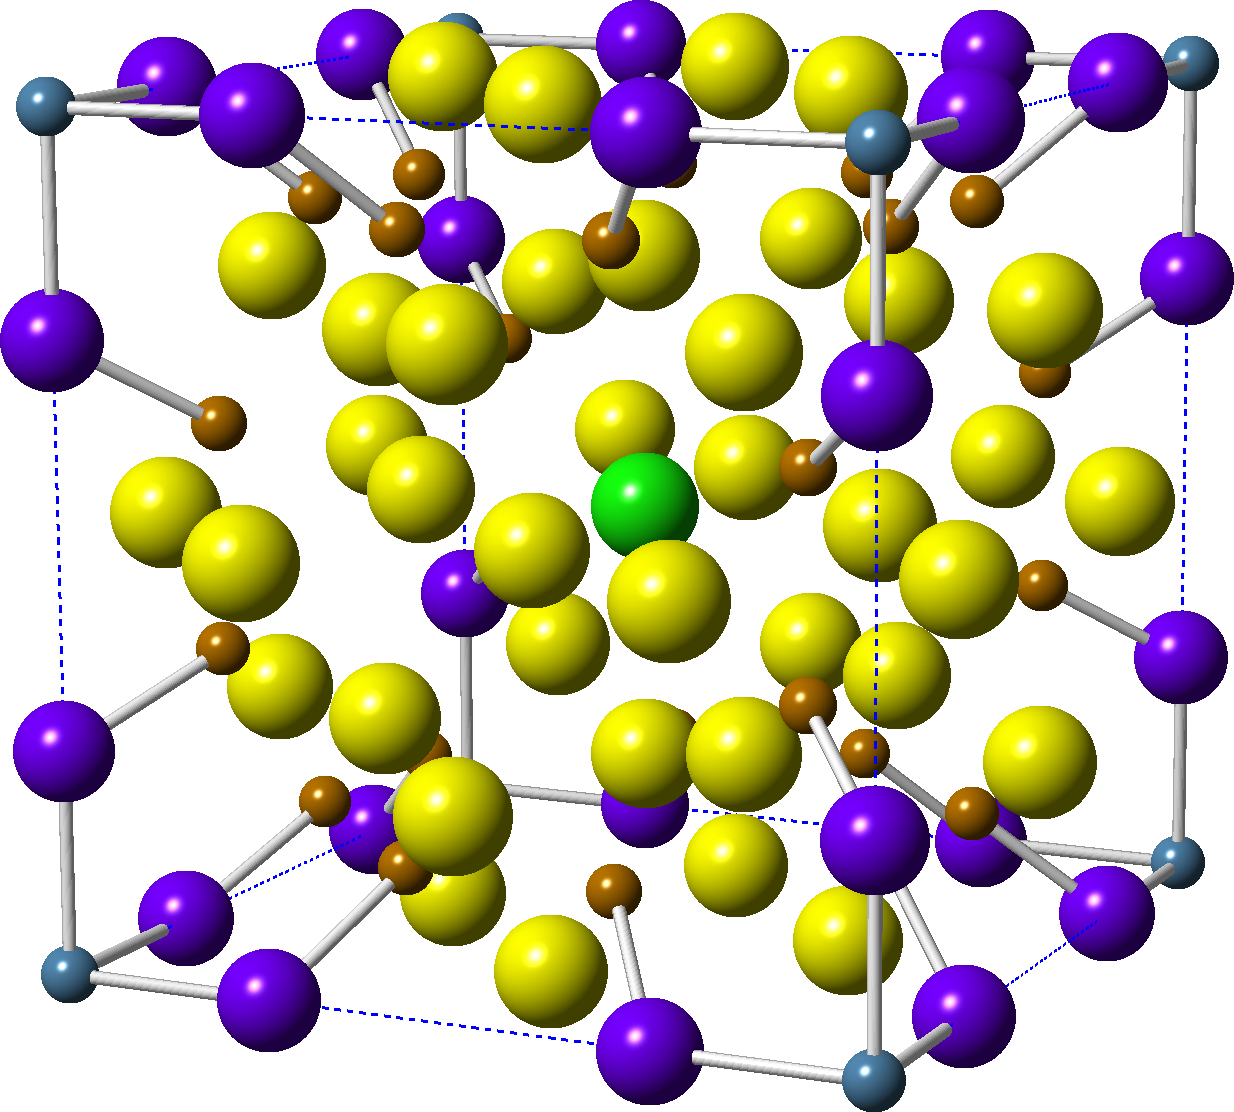
\includegraphics[height = 0.25\textwidth]{img/589-sol-4}}%
		{\caption{\texttt{0@a1,1@e1}($E = 0.0750$)}}
\end{subfloatrow}}{\caption[“0000589”的典型解]{%
	“0000589”的典型解(均已转换到使 \ce{Cl-} 在 $b$ 位置)%
}\label{fig:589-sol}}
\end{figure}

至此我们已经求解了 4 个测试结构。显然,如果只是手动输入(或复制、粘贴)第
\ref{ssec:decr-base} 小节中的命令并加以修改,这样会是十分低效且容易出错的。
在观察上述求解过程后,我们不难将其一般模式抽象为如下的 shell 脚本\footnote{%
	限于主题和篇幅,本文不试图对 shell 脚本编程进行详尽的解释;
	不熟悉相关背景的用户可以参考文献\parencite{robbins2005}。%
}(此处命名为 \verb|solve.sh|):
\begin{Verbatim}
\cm{#!/bin/sh}
decr_utils comb "$1" > combs.list
decr_utils dump "$1" < combs.list > crysts.list
decr_utils stat stat.sh hosts.conf < crysts.list > crysts.stat
decr_utils optim optim.sh hosts.conf < crysts.stat > crysts.optim
sort -k7g < crysts.optim > crysts.tmp && mv crysts.tmp crysts.optim
decr_utils merge "$1" < combs.list
\end{Verbatim}
这样只须将 \verb|hosts.conf| 复制到当前目录,便可通过以下命令求解:
\begin{Verbatim}
\cm{$} /path/to/solve.sh /path/to/some-cryst.txt
\end{Verbatim}
利用助手脚本(参考第 \ref{ssec:decr-arch} 小节)可以实现更加复杂的
自动化结构测定,相关内容将在第 \ref{sec:decr-adv} 节展示。

\subsection{EPC 筛选:以“0000428”和“0000219”结构为例}\label{ssec:epc-rank}

“0000428”结构($R\bar3$)的 decr 文件如下所示:
\begin{Verbatim}
\cm{# sg, abc, angles; ctl, extra; limits.}
148a	12.868 12.868 9.821	90 90 120
0.25 0.75 0.875	0.5 1.0
--

\cm{# rad/asf, n, limits, comb.}
Pb2+	18	--	--
Cr6+;Cr3+	3	--	--
O2-	24	--	--
Cl1-	18	--	--
\cm{# zooms.}
2:1-1

\cm{# 2theta, fwhm, hkl, mult, val.}
12.01	0.1	1 0 1	6	20.45
13.76	0.1	1 1 0	6	45.28
\cm{# (... further lines omitted ...)}
\end{Verbatim}
该结构的总 EPC 数为 88,单个 EPC 维数为 7--10,使用第 \ref{ssec:decr-auto} 小节
中的 \verb|solve.sh| 脚本求解时单次执行耗时约 \SI{25}{s}。虽然这个结构看似简单,
但是其求解并不十分直接,其中最重要的是直接使用 \verb|solve.sh| 时结果的重复性
出人意料地低:各 EPC 的排名并不稳定,且各 EPC 所得解的 $E$ 值浮动也较大;
根据本人的经验,这种情况通常是在维数大约为 15 的 EPC 中开始出现。无论如何,
在多次执行 \verb|solve.sh| 之后,不难发现排名最靠前的是以下 3 对等价 EPC%
($(0, 0, 1/2)$ 平移可使 $a/b$、$d/e$ 位置互变并保持其它 Wyckoff 记号不变):
\begin{itemize}
\item \verb|0@f1,1@a1,2@c1f1,3@f1|、\verb|0@f1,1@b1,2@c1f1,3@f1|:\\
	典型 $E$ 值为 0.057--0.060、0.064--0.066、0.075--0.100 或更大。
\item \verb|0@f1,1@a1,2@b1c2d1,3@f1|、\verb|0@f1,1@b1,2@a1c2e1,3@f1|:\\
	典型 $E$ 值为 0.097--0.099、0.103--0.121 或更大。
\item \verb|0@f1,1@a1,2@b1c2e1,3@f1|、\verb|0@f1,1@b1,2@a1c2d1,3@f1|:\\
	典型 $E$ 值为 0.113--0.114、0.120--0.125、0.162--0.168 或更大。
\end{itemize}
事实上,只须执行几次脚本便可注意到 \verb|1@a1,2@c1f1,...| 和
\verb|1@b1,2@c1f1,...| 所得解的最佳 $E$ 值明显低于其它两对 EPC,因此正确的
EPC 无疑是这一对。收集其各 $E$ 值的解,可发现 $E \geq 0.075$ 的解较为多样
(例如图 \ref{fig:428-sol}(c) 中的解),但 $E \in [0.064, 0.066]$ 的解(图
\ref{fig:428-sol}(b))和 $E \leq 0.060$ 的解(图 \ref{fig:428-sol}(a))基本
固定。考虑到后两个解从成键上看没有明显的问题,正确解应该是 $E$ 值最小的。

\begin{figure}[htbp!]\bfcmd
\ffigbox{\begin{subfloatrow}[3]
	\setlength{\columnsep}{-0.5em}
	\ffigbox[\FBwidth]{%
		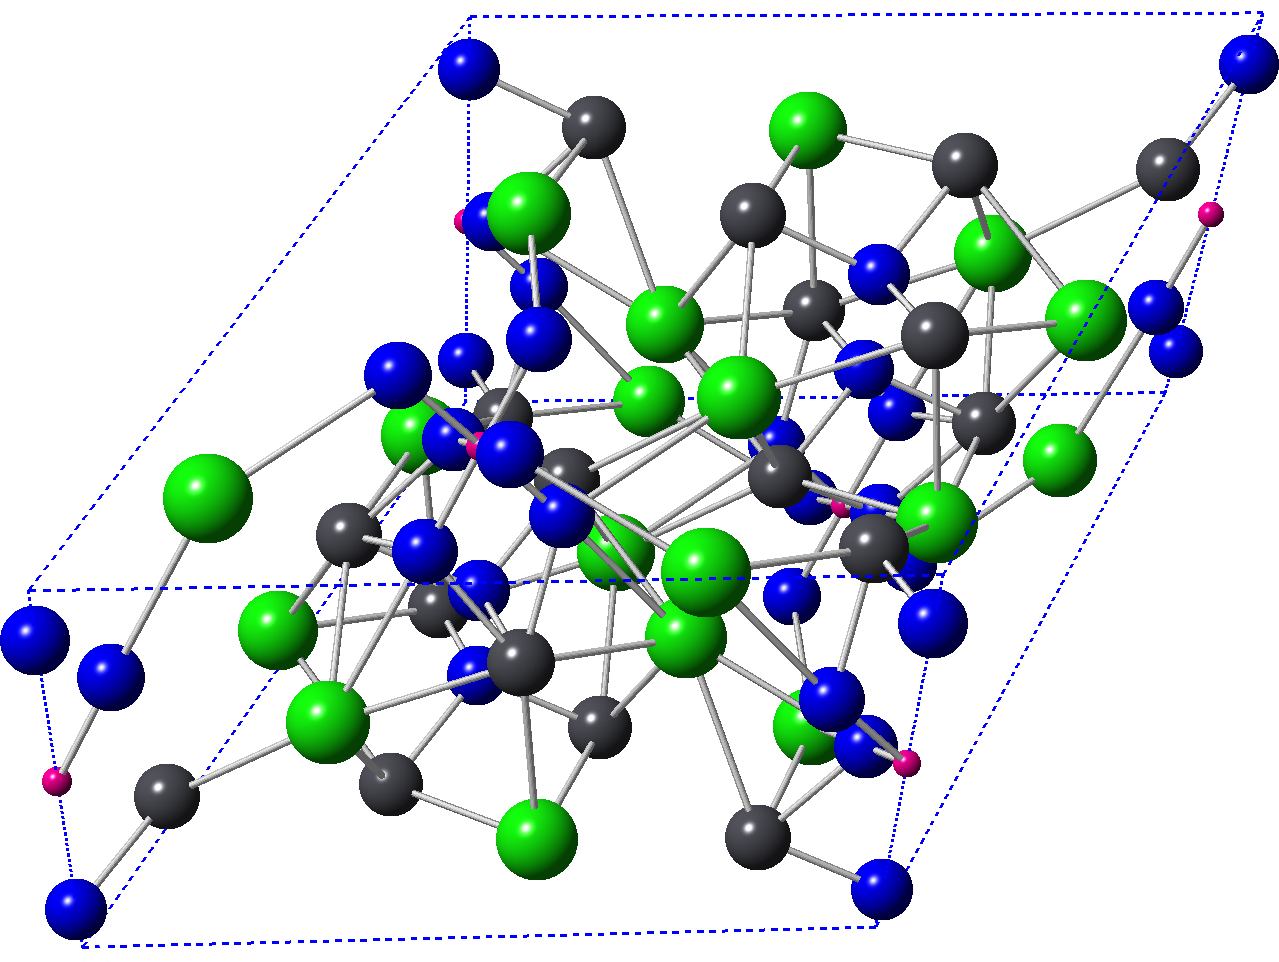
\includegraphics[width = 0.33\textwidth]{img/428-sol-1}%
	}{\caption{$R = 0.0586$}}
	\ffigbox[\FBwidth]{%
		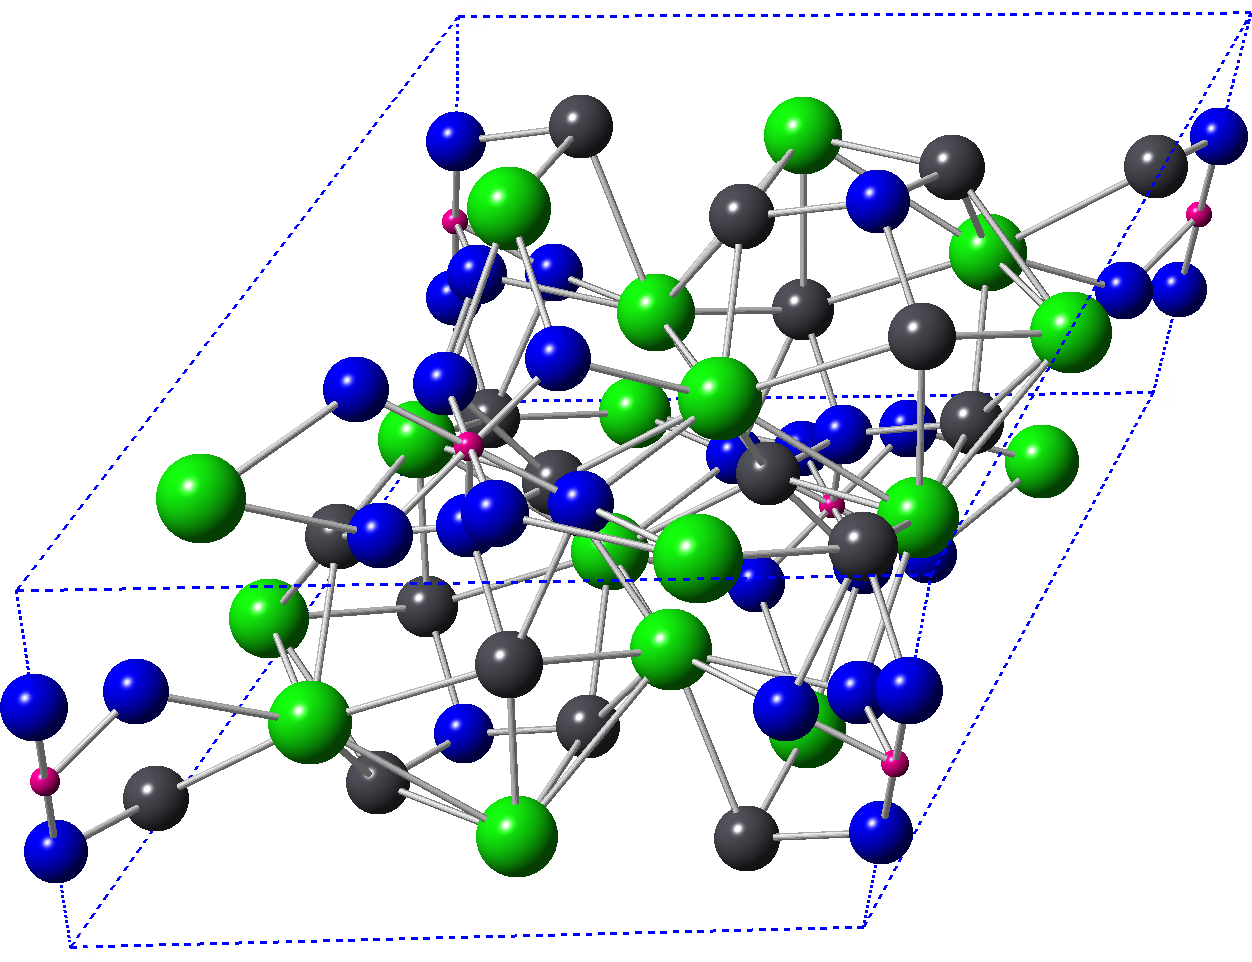
\includegraphics[width = 0.33\textwidth]{img/428-sol-2}%
	}{\caption{$R = 0.0650$}}
	\ffigbox[\FBwidth]{%
		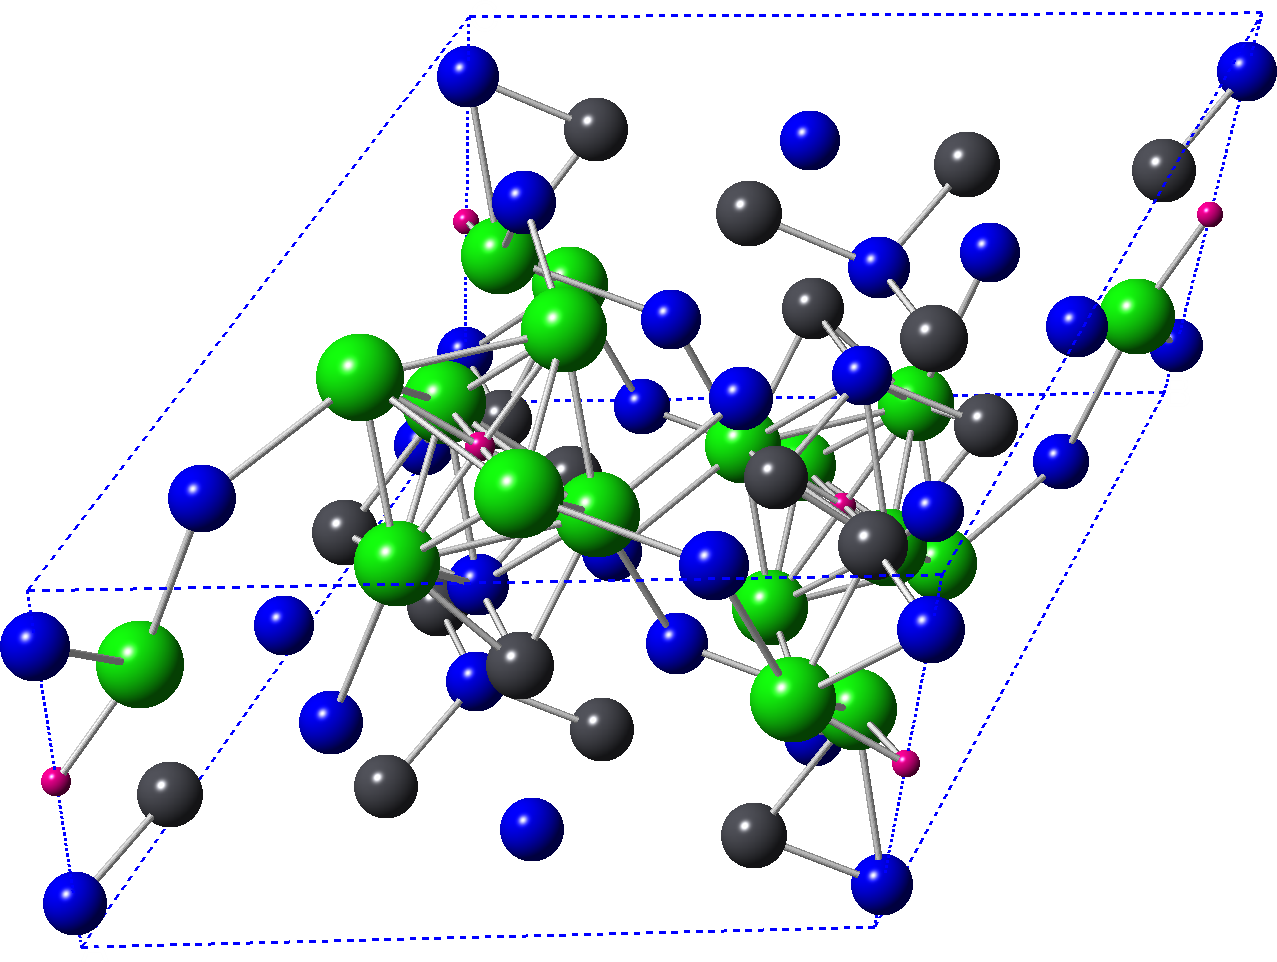
\includegraphics[width = 0.33\textwidth]{img/428-sol-3}%
	}{\caption{$R = 0.0801$}}
\end{subfloatrow}}{\caption[“0000428”的几个解]{%
	“0000428”的几个解,其中 (c) 只是相应 $E$ 值区间多种典型解中的一个%
}\label{fig:428-sol}}
\end{figure}

“0000219”结构(原数据采用的是 $Pbna$ 表示,求解前已转换\footnote{%
	可以使用 Bilbao 晶体学服务器\parencite{aroyo2006}上的 \texttt{SETSTRU}
	工具在同一空间群的不同表示之间转换,此外须特别注意 $hkl$ 和晶胞参数都需要
	转换。顺便值得一提的是,用此工具还可以对独立原子的 Wyckoff 位置进行判断,
	从而方便计算测试结构的晶胞化学式,以及寻找独立原子在 \emph{decryst}
	所用不对称单元内等效原子的坐标。%
}到 $Pbcn$)的 decr 文件如下所示:
\begin{Verbatim}
\cm{# sg, abc, angles; ctl, extra; limits.}
60	8.536 9.404 9.973	90 90 90
0.25 0.75 0.875	0.5 1.0
--

\cm{# rad/asf, n, limits, comb.}
P5+;P	8	--	--
Fe3+	12	--	--
O2-	44	--	--
\cm{# zooms.}
2:0-0	1.2:1-1	1.5:0-1

\cm{# 2theta, fwhm, hkl, mult, val.}
14.01	0.1	1 1 0	4	3.05
16.61	0.1	1 1 1	8	18.09
\cm{# (... further lines omitted ...)}
\end{Verbatim}
容易发现,原封不动地使用上述 \verb|solve.sh| 脚本求解须花费很长时间(约
\SI{1.5}{\hour}),这不难理解:观察 \verb|crysts.list| 可见虽然总 EPC
数不大(284),但是单个 EPC 的维数并不低(14--23),这导致每个 EPC
(特别是那些接近或超过 20 维的)须要花费很长的时间来求解。在这样的
情况下,我们可以根据统计分析的结果对 EPC 进行筛选:中断求解\footnote{%
	EPC 的维数对统计分析耗时的影响较小,因此我们来得及获取统计分析的结果。%
},并执行以下命令
\begin{Verbatim}
\cm{$} awk '\lb{} print 1 " " (1 / $7 + 10 * $6 / $5) "\bs{}t" $0 \rb{}' \bs
	< crysts.stat > crysts.rank0
\end{Verbatim}
来根据 \emph{EPCryst}\parencite{deng2011}中使用的经验公式计算各 EPC
的品质因数(FOM)。观察 \verb|crysts.rank0| 可发现各 EPC 的 FOM
并没有非常明显的聚类现象,因此我们先尝试对前 $1/4$ 的 EPC 求解:
\begin{Verbatim}
\cm{$} sed 70q < crysts.rank0 | cut -f 2-3 > crysts.stat
\cm{$} decr_utils optim optim.sh hosts.conf < crysts.stat > crysts.optim
\cm{$} sort -k7g < crysts.optim > crysts.tmp && mv crysts.tmp crysts.optim
\cm{$} decr_utils merge /path/to/0000219.txt < combs.list
\end{Verbatim}
观察 \verb|crysts.optim|,可见最佳 EPC 通常大致如下(注意 $(0, 1/2, 0)$
平移可使 $Pbcn$ 空间群中 $a/b$ 位置互变并保持其它 Wyckoff 记号不变):
\begin{Verbatim}
\cm{>} [...] 0.637264 0.0639186 0.0296934	0@d1,1@a1d1,2@c1d5.cr
\cm{>} [...] 0.638173 0.0653523 0.0484107	0@d1,1@b1d1,2@c1d5.cr
\cm{>} [...] 0.637305 0.0693133 0.0834741	0@d1,1@c1d1,2@b1d5.cr
\cm{>} [...] 0.638933 0.0675984 0.0847271	0@d1,1@c1d1,2@a1d5.cr
\cm{>} ...
\end{Verbatim}
于是可知只有 \verb|0@d1,1@a1d1,2@c1d5|、\verb|0@d1,1@b1d1,2@c1d5| 这对等价
EPC 是正确的;在可视化软件中查看 $E$ 值为 0.0297 和 0.0484 的两个解模型(图
\ref{fig:219-sol}),可见后者主要是部分 \ce{O^{2-}} 原子在 $c$ 方向上发生了
违背成键规律的较大偏移。加入以上 EPC 筛选之后,求解所需时长可以压缩到约
\SI{45}{\minute}(只压缩了约 $1/2$ 的时间,因为筛选出的 EPC 多为 18--22 维)。

\begin{figure}[htbp!]\bfcmd
\ffigbox{\begin{subfloatrow}
	\setlength{\columnsep}{2em}
	\ffigbox[\FBwidth]%
		{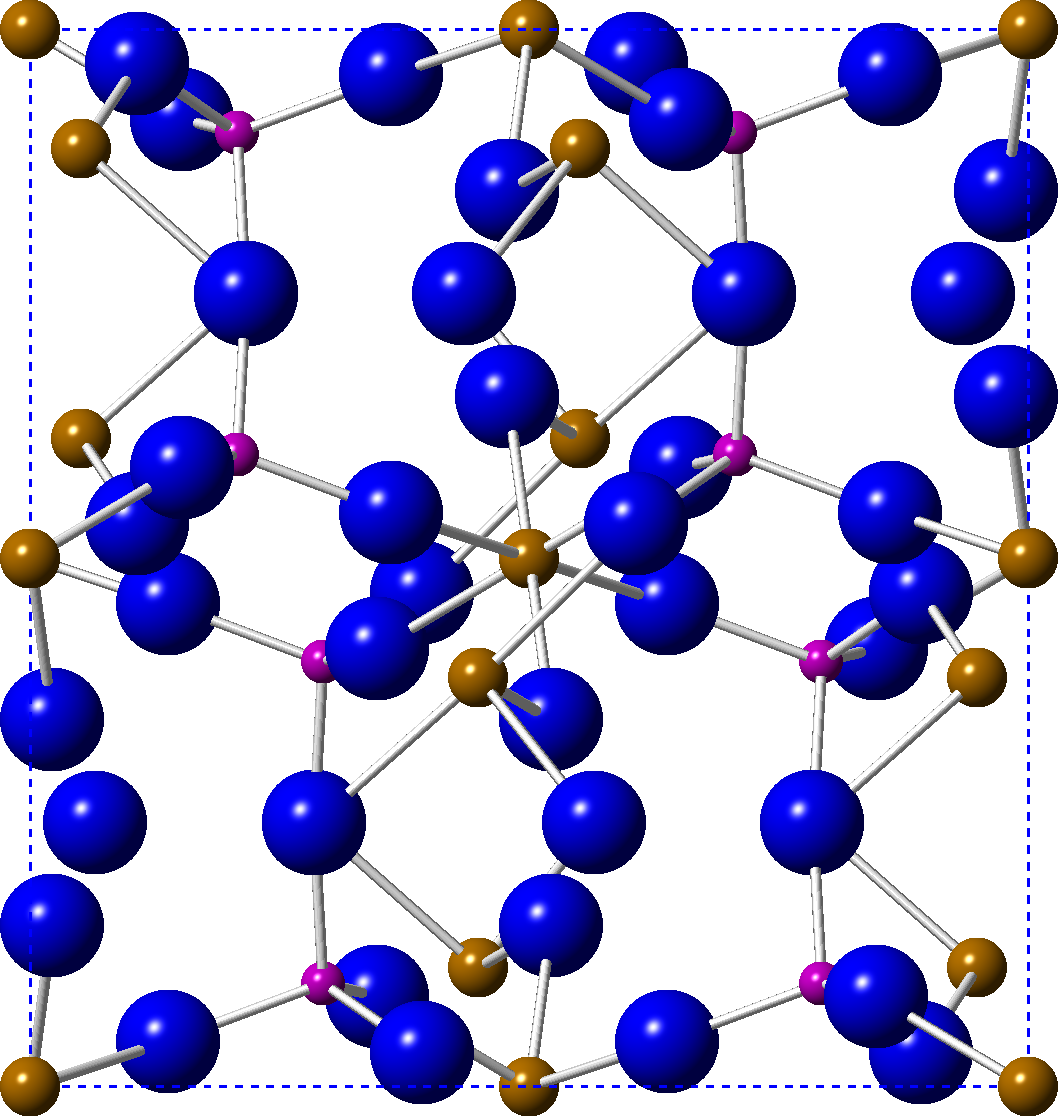
\includegraphics[width = 0.25\textwidth]{img/219-sol-1}}%
		{\caption{$E = 0.0297$}}
	\ffigbox[\FBwidth]%
		{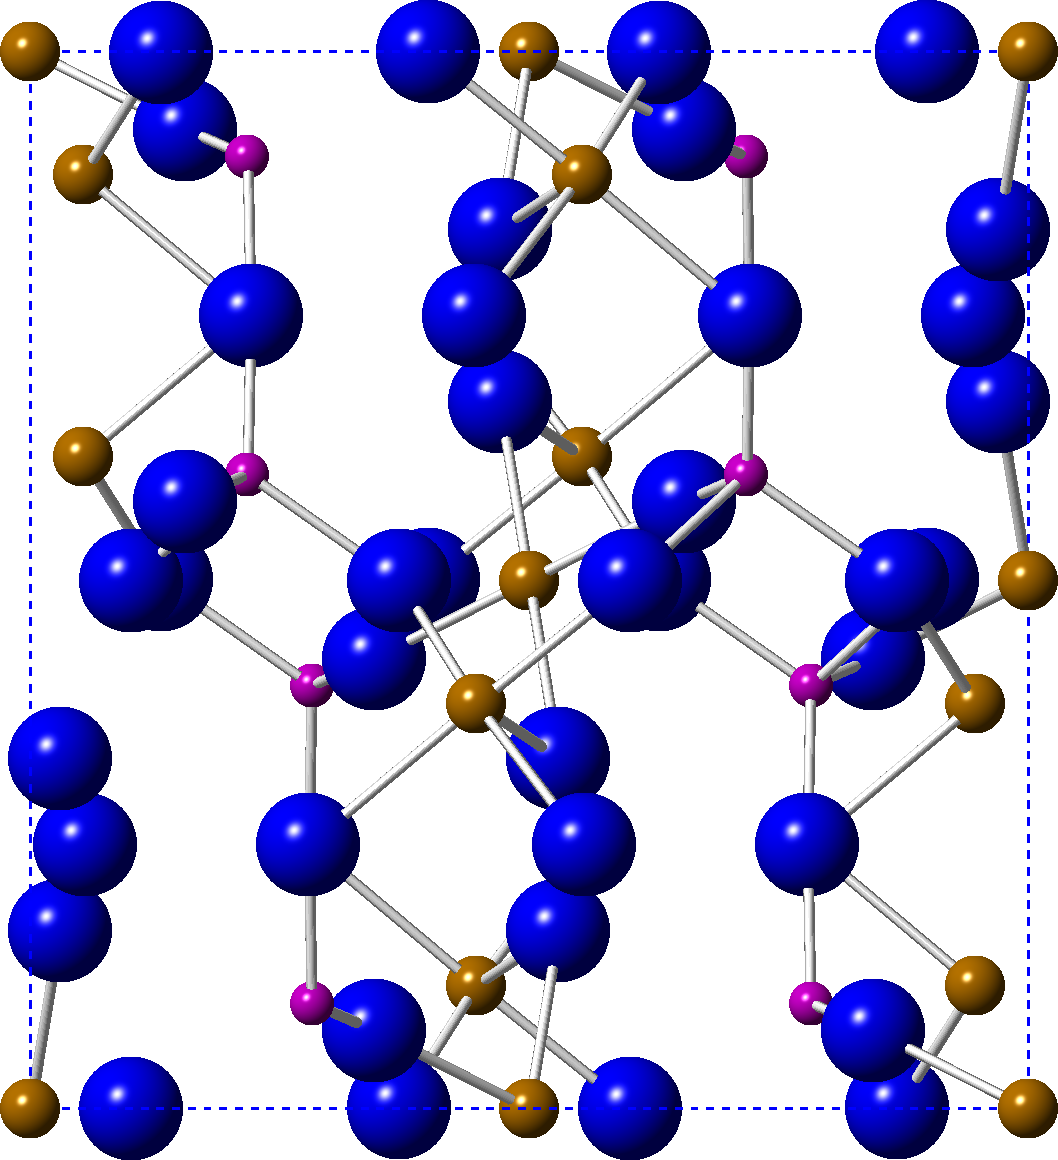
\includegraphics[width = 0.25\textwidth]{img/219-sol-2}}%
		{\caption{$E = 0.0484$}}
\end{subfloatrow}}{\caption[“0000219”典型解在 $a$ 方向上的投影]{%
	“0000219”典型解在 $a$ 方向上的投影
	(均已转换到使部分 \ce{Fe^{3+}} 在 $a$ 位置)%
}\label{fig:219-sol}}
\end{figure}

这里有必要强调,本章所有求解均是在启用了 Intel i7-3720QM CPU 的所有 8 个处理器
线程的前提下进行的:在求解其它结构时这或许不是必需,但在求解“0000219”时可以
看到,因为 EPC 任务是完美并行的(参考第 \ref{ssec:decr-para} 小节),所以我们
利用并行节省了大约 $0.75 \times 7 = \SI{5.2}{\hour}$ 的时间,这是不可忽视的。
可能有读者会疑惑,在硬件性能突飞猛进的当代,从软件方面提升计算效率是否仍有
必要?事实上,根据近年来 CPU 性能的增长趋势(图 \ref{fig:fp-perf}),%
CPU 的单线程浮点性能大约是每 12 年提升一个数量级,所以数倍的性能提升
仍然具有重要意义,何况在单线程性能增长放缓的背景之下大力发展
并行和分布式计算本来就是科学计算(乃至通用计算)的大势所趋。

\begin{figure}[htbp!]
\ffigbox{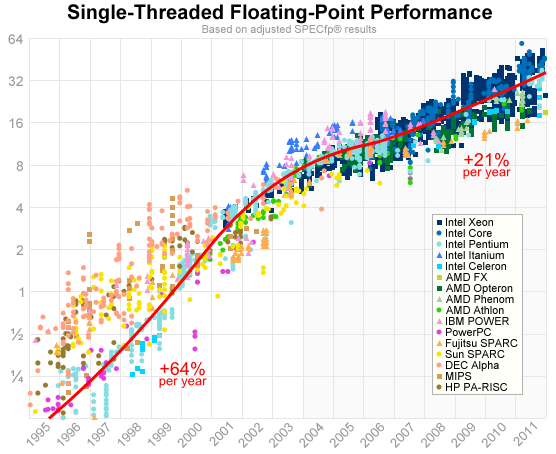
\includegraphics[width = 0.75\textwidth]{img/fp-perf}}{\caption[%
	CPU 单线程浮点性能在 1995--2011 年间的增长%
]{%
	CPU 单线程浮点性能在 1995--2011 年间的增长
	(图引自文献 (\cite{preshing2012}))%
}\label{fig:fp-perf}}
\end{figure}

\section{\emph{decryst} 的高级用法和常用技巧}\label{sec:decr-adv}

在本节中,第 \ref{ssec:heavy-atom} 小节将演示如何利用 \emph{decryst} 的自动化
机制实现正空间法中的重原子法,而重原子法是之后各小节中结构测定的基础。第
\ref{ssec:epc-search} 小节将演示如何实现对重原子、轻原子等效点系组合(EPC)
的分步确定,以及在此之后如何自动化地对同时涉及轻、重原子的 EPC 进行准确的求解。
第 \ref{ssec:epc-filter} 小节将演示对 EPC 的复杂筛选:其中不仅会用到之前的
EPC 筛选方法,而且会在结构测定的各个步骤中多次利用原子重叠评估函数(参考第
\ref{ssec:eval-func} 小节)对 EPC 进行精细的筛选。

\subsection{重原子法:以 \ce{PbSO4} 为例}\label{ssec:heavy-atom}

\ce{PbSO4}(原数据采用的是 $Pbnm$ 表示,求解前已转换到 $Pnma$)的
decr 文件(假设文件名为 \verb|pso.txt|)如下所示:
\begin{Verbatim}
\cm{# sg, abc, angles; ctl, extra; limits.}
62	8.4720 5.3973 6.9549	90 90 90
0.25 0.75 0.875	0.5 1.0
--

\cm{# rad/asf, n, limits, comb.}
Pb2+	4	--	--
S6+;S	4	--	--
O2-	16	--	--
\cm{# zooms.}
1.4:1-0	2.8:1-1
0.9:2-1

\cm{# 2theta, fwhm, hkl, mult, val.}
16.49	0.2	1 0 1	4	2.70
20.83	0.2	0 1 1	4	79.73
\cm{# (... further lines omitted ...)}
\end{Verbatim}

\ce{PbSO4} 结构可以直接使用第 \ref{ssec:decr-auto} 小节中的 \verb|solve.sh|
脚本求解,耗时约 \SI{8}{\second};然而考虑到 \ce{PbSO4} 中 \ce{Pb^{2+}} 和
\ce{S^{6+}} 均明显地重于 \ce{O^{2-}},该结构的简单性使其在演示重原子法时
成为一个完美的例子。为了使用重原子法求解 \ce{PbSO4} 结构,我们首先须要使
\emph{decryst} 忽略 \ce{O^{2-}} 原子,这可以通过注释实现:
\begin{Verbatim}
\cm{$} sed -i '/^O2-/ s/^/#/; /:2-/ s/^/#/' pso.txt
\end{Verbatim}
注意原 \verb|decr| 文件中以 \verb|O2-| 开头的行只有指定晶胞中 \ce{O^{2-}}
个数的行,且该文件中包含 \verb|2:| 字符串的数据行只有指定和 \ce{O^{2-}}
相关对缩放因子的行,因此以上命令能够精准地注释掉所有涉及 \ce{O^{2-}}
的数据行。由于重原子法须要分步求解重、轻原子,为了避免不同步骤中的
文件互相覆盖,我们可以在不同目录中生成不同步骤所需的文件:
\begin{Verbatim}
\cm{$} mkdir ps
\cm{$} decr_utils comb pso.txt | awk '\lb print "ps/pso," $0 \rb' |
	decr_utils dump pso.txt > ps/index.list
\end{Verbatim}

在 \verb|ps| 目录中生成 cryst 文件和 crysts 文件之后,
便可以对各 EPC 进行统计分析和全局最优化:
\begin{Verbatim}
\cm{$} PYTHONUNBUFFERED=1 decr_utils stat stat.sh hosts.conf < ps/index.list |
	tee ps/index.tmp | do_rank.sh 0 > ps/index.rank0
\cm{$} grep -v '^#' < ps/index.rank0 | cut -f 2-3 |
	PYTHONUNBUFFERED=1 decr_utils optim optim.sh hosts.conf |
	tee ps/index.tmp | do_rank.sh 1 > ps/index.rank1
\end{Verbatim}
\verb|PYTHONUNBUFFERED| 环境变量强制 Python 将每一行结果分别输出而不是将若干行
结果凑到一起输出。助手脚本 \verb|do_rank.sh| 的作用是在 crysts 文件中添加两列
以记录各 EPC 的品质因数(FOM,基于 \emph{EPCryst}\parencite{deng2011}%
中的经验公式)以及是否零维,例如以下数据行(为了方便解释,
此处明确区分了代码中的空格和制表符)
\begin{Verbatim}[showtabs = true, showspaces = true]
\cm{>\ }0 0 - - - - 0.522904	ps/pso,0@b1,1@a1.cr
\cm{>\ }2 1000 200 0.01 0.396994 0.140564 0.129636	ps/pso,0@c1,1@a1.cr
\end{Verbatim}
将被变换为
\begin{Verbatim}[showtabs = true, showspaces = true]
\cm{>\ }0 3.82479	... - - 0.522904	ps/pso,0@b1,1@a1.cr
\cm{>\ }1 11.2546	... 0.396994 0.140564 0.129636	ps/pso,0@c1,1@a1.cr
\end{Verbatim}
\verb|do_rank.sh| 的命令行参数决定了其对数据行排序的方式:为 \verb|1| 时
只根据 FOM 排序,而为 \verb|0| 时将零维 EPC 排在前面,然后才是按 FOM 排序。
注意其中使用 \verb|grep| 命令去掉了 \verb|index.rank0| 中用“\verb|#|”
注释掉的行,从而避免对这些行计算上述的临时字段。此外,以上操作中
有规律地使用了空白字符(参考第 \ref{ssec:decr-fmt} 小节),
从而方便了之后使用 \verb|cut| 命令去掉上述临时字段;
这一技巧事实上已经在第 \ref{ssec:decr-auto} 小节中使用。

在求解完重原子的坐标之后,我们就可以导出结果了:
\begin{Verbatim}
\cm{$} do_filter.sh < ps/index.rank1 | decr_utils merge pso.txt > /dev/null
\end{Verbatim}
\verb|decr_utils| 在导出 decr 文件时会保留原有注释,
于是上一步中 \verb|pso.txt| 的片段
\begin{Verbatim}
\cm{#O2-}	\cm{16}	\cm{--}	\cm{--}
\cm{# Pairwise zoom factors.}
1.4:1-0 2.8:1-1
\cm{#0.9:2-1}
\end{Verbatim}
在正确 EPC 所对应的 decr 文件(\verb|ps/pso,0@c1,1@c1.cr|)中将被变换为
\begin{Verbatim}
\cm{#O2-}	\cm{16}	\cm{--}	\cm{--}
\cm{# Pairwise zoom factors.}
1.4:1-0 2.8:1-1
\cm{#0.9:2-1}
0@c1	0.314226	0.25	0.33363
1@c1	0.43269	0.25	0.805449
\end{Verbatim}
因此为了求解 \ce{O^{2-}} 原子的位置,我们只须去掉所有涉及 \ce{O^{2-}} 的注释:
\begin{Verbatim}
\cm{$} sed -i '/^#O2-/ s/^#//; /:2-/ s/^#//' pso.txt
\cm{$} do_filter.sh < ps/index.rank1 | sed 's/\bs.cr$/.txt/' |
	xargs -n 100 sed -i '/^#O2-/ s/^#//; /:2-/ s/^#//'
\end{Verbatim}
其中 \verb|do_filter.sh| 的作用是提取 \verb|rank|
文件中未被注释的 cryst 文件名,例如
\begin{Verbatim}
\cm{> #0 3.82479}	\cm{... - - 0.522904}	\cm{ps/pso,0@b1,1@a1.cr}
\cm{>} 1 11.2546	... 0.396994 0.140564 0.129636	ps/pso,0@c1,1@a1.cr
\end{Verbatim}
将被变换为
\begin{Verbatim}
\cm{>} ps/pso,0@c1,1@a1.cr
\end{Verbatim}

接下来我们须要产生 \ce{O^{2-}} 原子的 EPC:
\begin{Verbatim}
\cm{$} mkdir pso
\cm{$} do_filter.sh < ps/index.rank1 | sed 's/\bs.cr$/.txt/' | while read f; do
	decr_utils comb "$f" | awk '\lb
	     print "pso/'"$(basename $f | sed -r 's@\bs.[^/.]+$@,@')"'" $0
	\rb' | decr_utils dump "$f" >> pso/index.list; done
\end{Verbatim}
以上第 2 行命令的作用是将从重原子 EPC 所对应 decr 文件生成的 cryst 文件冠以
相应重原子 EPC 的前缀:例如从 \verb|ps/pso,0@c1,1@c1.txt| 生成的 \verb|2@c1d1|
cryst 文件将被保存到 \verb|pso/pso,0@c1,1@c1,2@c1d1.cr|;通过这一操作,
我们事实上得到了(包含所有原子的)总 EPC 的完整表达式。\ce{O^{2-}}
原子的统计分析和全局最优化步骤和之前如出一辙,不再赘述:
\begin{Verbatim}
\cm{$} PYTHONUNBUFFERED=1 decr_utils stat stat.sh hosts.conf < pso/index.list |
	tee pso/index.tmp | do_rank.sh 0 > pso/index.rank0
\cm{$} grep -v '^#' < pso/index.rank0 | cut -f 2-3 |
	PYTHONUNBUFFERED=1 decr_utils optim optim.sh hosts.conf |
	tee pso/index.tmp | do_rank.sh 1 > pso/index.rank1
\cm{$} do_filter.sh < pso/index.rank1 | decr_utils merge pso.txt > /dev/null
\cm{$} rm ps/index.tmp pso/index.tmp
\end{Verbatim}
除去人工步骤之后,以上求解过程总耗时约 \SI{5}{\second}。

\subsection{实际 EPC 的搜索:以“0000158”结构为例}\label{ssec:epc-search}

第 \ref{ssec:heavy-atom} 小节中求解 \ce{PbSO4} 结构所用的命令行操作具有很强的
典型性:许多代码在其它结构的求解中只需很少修改就可以使用,这些代码被抽象为了
助手脚本;在使用助手脚本之后,\ce{PbSO4} 结构的求解可以用以下脚本实现:
\begin{Verbatim}
\cm{#!/bin/sh}
sed -i '/^O2-/ s/^/#/; /:2-/ s/^/#/' pso.txt
mkdir ps
echo pso.txt | do_dump.sh ps
do_stat.sh ps && do_optim.sh ps && do_merge.sh pso.txt ps
sed -i '/^#O2-/ s/^#//; /:2-/ s/^#//' pso.txt
do_filter.sh < ps/index.rank1 | sed 's/\bs.cr$/.txt/' |
	xargs -n 100 sed -i '/^#O2-/ s/^#//; /:2-/ s/^#//'
mkdir pso
do_filter.sh < ps/index.rank1 | sed 's/\bs.cr$/.txt/' | do_dump.sh pso
do_stat.sh pso && do_optim.sh pso && do_merge.sh pso.txt pso
rm ps/index.tmp pso/index.tmp
\end{Verbatim}
可能有读者会感到疑惑:脚本一般是用于自动化地运行具有重复性的任务,但晶体
结构在解出之后一般不用重复求解,那么这样的求解脚本有什么意义?事实上,
因为实际结构的求解往往是相当复杂的,其步骤和参数往往需要多次调整;因此,
求解脚本不仅可以方便用户在调整求解步骤和参数时对求解的全程进行宏观的把握,
而且可以作为增强求解过程可重复性的“实验记录”,从而为其它结构的求解提供参考。
事实上,本节中后两种结构的求解都是以上述 \ce{PbSO4} 求解脚本为基础的。

“0000158”结构($C2/c$)的 decr 文件(假设文件名为 \verb|158.txt|)如下所示:
\begin{Verbatim}
\cm{# sg, abc, angles; ctl, extra; limits.}
15a	10.129 8.306 8.533	90 112.19 90
0.25 0.75 0.875	0.5 1.0
--

\cm{# rad/asf, n, limits, comb.}
Ca2+	4	--	--
S6+;S	8	--	--
Na1+	8	--	--
O2-	32	--	--
\cm{# zooms.}
2.8:1-1
1.2:2,0-1

\cm{# 2theta, fwhm, hkl, mult, val.}
14.24	0.1	1 1 0	4	44.67
18.92	0.1	2 0 0	2	23.65
\cm{# (... further lines omitted ...)}
\end{Verbatim}
该结构的总 EPC 数为 3706,单个 EPC 维数为 9--19;注意到其中的原子可以分为重原子
\ce{S^{6+}}、\ce{Ca^{2+}} 和轻原子 \ce{Na+}、\ce{O^{2-}},其可以使用重原子法
求解以节约时间,因此我们首先求解重原子(EPC 数为 44,单个 EPC 维数为 0--4):
\begin{Verbatim}
\cm{$} sed -ri '/^(O2-|Na1\bs+)/ s/^/#/; /:2,/ s/^/#/' 158.txt
\cm{$} mkdir cs
\cm{$} echo 158.txt | do_dump.sh cs
\cm{$} do_stat.sh cs && do_optim.sh cs && do_merge.sh 158.txt cs
\end{Verbatim}

观察 \verb|cs/index.rank1|,不难注意到 \verb|0@e1,1@f1| 是唯一合理的重原子 EPC:
其 $E$ 值为 0.20 左右,其它非零维 EPC 的 $E$ 值都在 0.30--0.40 之间,而所有零维
EPC 的 $E$ 值都大于 0.40。因此我们在求解轻原子时只采用 \verb|0@e1,1@f1|
这一重原子 EPC(下属 EPC 数为 350,单个 EPC 维数为 6--15):
\begin{Verbatim}
\cm{$} sed -i '2,$ s/^/#/' cs/index.rank1
\cm{$} sed -ri '/^#(O2-|Na1\bs+)/ s/^#//; /:2,/ s/^#//' 158.txt
\cm{$} do_filter.sh < cs/index.rank1 | sed 's/\bs.cr$/.txt/' |
	xargs -n 100 sed -ri '/^#(O2-|Na1\bs+)/ s/^#//; /:2,/ s/^#//'
\cm{$} mkdir no
\cm{$} do_filter.sh < cs/index.rank1 | sed 's/\bs.cr$/.txt/' | do_dump.sh no
\cm{$} do_stat.sh no && do_optim.sh no && do_merge.sh 158.txt no
\end{Verbatim}
观察 \verb|no/index.rank1| 可见各 EPC 的 $E$ 值没有明显的聚类现象,所以求解似乎
失败了,但事实并非如此:在“0000158”中,重原子 \ce{S^{6+}}、\ce{Ca^{2+}} 和轻原子
\ce{Na+}、\ce{O^{2-}} 的电子数相差并不悬殊,因此对重、轻原子分别求解得不到很满意
的结果并不难理解。然而从直觉上不难理解分别求解得到的(包含所有原子的)总 EPC
排名和直接对所有原子求解得到的总 EPC 排名仍会存在一定的相关性,因此我们可以对
排名靠前的总 EPC 再次进行求解(这里取了前 30 个;此外注意 \verb|do_dump.sh| 生成
的 cryst 文件名包含了总 EPC 的完整表达式,参考第 \ref{ssec:heavy-atom} 小节):
\begin{Verbatim}
\cm{$} sed -i '31,$ s/^/#/' no/index.rank1
\cm{$} mkdir csno
\cm{$} do_filter.sh < no/index.rank1 | sed 's@^[^,]\bs+,@@; s/\bs.cr//' |
	awk '\lb print "csno/158," $0 ".cr\bs{}t" $0 \rb' |
	decr_utils dump 158.txt > csno/index.list
\cm{$} do_stat.sh csno && do_optim.sh csno && do_merge.sh 158.txt csno
\end{Verbatim}

观察 \verb|csno/index.rank1| 可见正确 EPC \verb|0@e1,1@f1,2@f1,3@f4| 是
唯一合理的 EPC:其 $E$ 值最多为 0.05 左右,而其它 EPC 的 $E$ 值都至少为 0.13
左右。注意到该 EPC 的维数为 19,我们须要多次进行全局最优化,然后挑选最优解:
\begin{Verbatim}
\cm{$} mkdir fin
\cm{$} l="$(sed 1q < csno/index.rank1 | sed 's/csno/fin/; s/\.cr$//')"
\cm{$} name="$(echo "$l" | cut -f 3 | sed 's@.*/@@')"
\cm{$} for i in $(seq 0 9); do
	cp csno/"$name".cr fin/"$name-$i".cr
	echo "$l-$i".cr >> fin/index.rank0; done
\cm{$} do_optim.sh fin && do_merge.sh 158.txt fin
\cm{$} rm */index.tmp
\end{Verbatim}
\verb|fin/index.rank1| 中排名最靠前的一般会是 3 个左右的 $E$ 值在 0.025--0.030
的解,这些就是正确解;除去人工步骤之后,以上求解过程总耗时约 \SI{5}{\minute}。

\subsection{EPC 的复杂筛选:以“0009563”结构为例}\label{ssec:epc-filter}

“0009563”结构($P\bar3c1$)的 decr 文件(假设文件名为 \verb|0009563.txt|)
如下所示(为了方便解释,此处明确区分了代码中的空格和制表符):
\begin{Verbatim}[showtabs = true, showspaces = true]
\cm{# sg, abc, angles; ctl, extra; limits.}
165	12.19 12.19 10.14	90 90 120
0.25 0.75 0.875	0.5 1.0
--

\cm{# rad/asf, n, limits, comb.}
Rb1+	12	--	--
Ge4+	18	--	--
Ti4+	6	--	--
O2-	54	--	--
\cm{# zooms.}
1.5:1,2-1,2

\cm{# 2theta, fwhm, hkl, mult, val.}
16.97	0.2	1 1 1	12	10.71
17.49	0.2	0 0 2	2	7.14
\cm{# (... further lines omitted ...)}
\end{Verbatim}
本小节的详细测试结果(包括图 \ref{fig:9563-sol} 所对应的结构数据)可以从文献%
\parencite{liu2018}的补充材料中获取。注意到“0009563”中的金属原子均明显重于
\ce{O^{2-}},使用重原子法求解是很合适的,因此本人首先生成了重原子的
cryst 文件(EPC 数为 1451 个,单个 EPC 维数为 5--8):
\begin{Verbatim}
\cm{$} mkdir rgt-0
\cm{$} sed '/^O2-/ s/^/#/; s/^0\bs.25 /0.99 /' < 0009563.txt > 9563.txt
\cm{$} echo 9563.txt | do_dump.sh rgt-0
\cm{$} mkdir rgt-1
\cm{$} sed -i 's/^0\bs.99 /0.25 /' 9563.txt
\cm{$} echo 9563.txt | do_dump.sh rgt-1
\end{Verbatim}
因为 EPC 数很大,我们须要尽量对其进行筛选,从而减少(包含所有原子的)总 EPC
备选范围。受\textcite{lu1965},\textcite{reddy1965}所做工作的启发,本人生成了
两套 cryst 文件,其中组合因子 $\mu$(参考第 \ref{ssec:decr-fmt} 小节)
的值分别为\footnote{%
	考虑到部分化学上很不合理的 EPC 可能以大概率产生原子重叠评估函数值 $B = 1$
	的晶体模型,不将 $\mu$ 值设定为 1 可以避免这些 EPC 的全局最优化过早结束。%
} 0.99 和默认的 0.25;通过对 $\mu = 0.99$ 的 cryst 文件进行全局最优化,
我们就可以筛除那些不可能产生无原子重叠晶体模型的 EPC。此外还须要强调的是
\verb|0009563.txt| 中在行首出现且后面跟着空格的数值只有 $\mu$ 值,
这是以上命令可以精准地对 $\mu$ 值进行更改的基础。

我们接下来会看到,即使事先筛除不可能产生无原子重叠晶体模型的 EPC,全局最优化
仍可能得到发生重叠的解模型;为了筛除这种解模型,本人定义了一个在 crysts
文件中加入原子重叠评估函数值 $B$ 的 shell 函数:
\begin{Verbatim}
\cm{$} do_bump_sh() \lb
	while read l; do
	name="$(echo "$l" | cut -f 3 | sed 's/\bs.cr$/.txt/')"
	echo 'nil.cr nil' | decr_utils dump "$name" > /dev/null
	sed 's/0\bs.25 0\bs.75 0\bs.875$/0.99 0.75 0.875/' < nil.cr |
	     decr_mcs 0 | cut -d ' ' -f 3 | tr '\bs{}n' ' '
	echo "$l"; done; \rb
\end{Verbatim}
其中 \verb|nil| EPC 的意义可以参考第 \ref{ssec:decr-fmt} 小节。接下来本人
按照上文所述的思路对之前产生的 cryst 文件进行了统计分析和全局最优化:
\begin{Verbatim}
\cm{$} do_stat.sh rgt-0 && do_optim.sh rgt-0
\cm{$} mv -f rgt-0/index.rank1 rgt-0/index.tmp
\cm{$} awk '\lb print ($9 > 0.12 ? "#" : "") $0 \rb' \bs
	< rgt-0/index.tmp > rgt-0/index.rank1
\cm{$} do_filter.sh < rgt-0/index.rank1 | sed 's@.*/@rgt-1/@' > rgt-1/index.tmp
\cm{$} grep -Ff rgt-1/index.tmp < rgt-1/index.list > rgt-1/index.tmpp
\cm{$} mv -f rgt-1/index.tmpp rgt-1/index.list
\cm{$} do_stat.sh rgt-1 && do_optim.sh rgt-1 && do_merge.sh 9563.txt rgt-1
\cm{$} do_bump_sh < rgt-1/index.rank1 | awk '\lb print
	($10 > 0.2 || $1 > 0.02 ? "#" : "") $0 \rb' > rgt-1/index.rank2
\end{Verbatim}
以上命令先筛除了 $\mu = 0.99$ 时解模型 $E > 0.12$ 的 EPC,剩下 183 个(13\%);
在恢复默认 $\mu$ 值后又筛除了解模型 $E > 0.2$ 的 EPC,剩下 26 个。本人在观察
\verb|index.rank2| 之后发现其中的 EPC 分为一组解模型 $B \leq 0.0027$ 的和一组
解模型 $B \in [0.056, 0.112]$ 的,并由此筛除了所有解模型 $B > 0.02$ 的 EPC,
剩下 20 个(11\%)。除去人工步骤之后,重原子 EPC 求解耗时约 \SI{2.5}{\minute}。
事实上,重原子求解得到了正确的结果:正确 EPC \verb|0@g1,1@f1g1,2@b1d1| 的
$E$ 值(0.058)是最小的;事后本人在可视化软件中查看重原子 EPC 的解模型,
确认了所有因 $B$ 值过大而被筛除的解模型中都发生了很明显的原子重叠。

仿照以上步骤,本人对 \ce{O^{2-}} 原子的 EPC 进行了求解:
\begin{Verbatim}
\cm{$} mkdir rgto-0 && sed -i '/^#O2-/ s/^#//; s/^0\bs.25 /0.99 /' 9563.txt
\cm{$} do_filter.sh < rgt-1/index.rank2 | sed 's/\bs.cr$/.txt/' |
	xargs -n 100 sed -i '/^#O2-/ s/^#//; s/^0\bs.25 /0.99 /'
\cm{$} do_filter.sh < rgt-1/index.rank2 |
	sed 's/\bs.cr$/.txt/' | do_dump.sh rgto-0
\cm{$} mkdir rgto-1 && sed -i 's/^0\bs.99 /0.25 /' 9563.txt
\cm{$} do_filter.sh < rgt-1/index.rank2 | sed 's/\bs.cr$/.txt/' |
	xargs -n 100 sed -i 's/^0\bs.99 /0.25 /'
\cm{$} do_filter.sh < rgt-1/index.rank2 |
	sed 's/\bs.cr$/.txt/' | do_dump.sh rgto-1
\cm{$} do_stat.sh rgto-0 && mv -f rgto-0/index.rank0 rgto-0/index.tmp
\cm{$} awk '\lb print ($9 > 0.99 ? "#" : "") $0 \rb' \bs
	< rgto-0/index.tmp > rgto-0/index.rank0
\cm{$} do_optim.sh rgto-0 && mv -f rgto-0/index.rank1 rgto-0/index.tmp
\cm{$} awk '\lb print ($9 > 0.05 ? "#" : "") $0 \rb' \bs
	< rgto-0/index.tmp > rgto-0/index.rank1
\cm{$} do_filter.sh < rgto-0/index.rank1 |
	sed 's@.*/@rgto-1/@' > rgto-1/index.tmp
\cm{$} grep -Ff rgto-1/index.tmp < rgto-1/index.list > rgto-1/index.tmpp
\cm{$} mv -f rgto-1/index.tmpp rgto-1/index.list
\cm{$} do_stat.sh rgto-1 && do_optim.sh rgto-1 && do_merge.sh 9563.txt rgto-1
\cm{$} do_bump_sh < rgto-1/index.rank1 |
	awk '\lb print ($1 > 0.02 ? "#" : "") $0 \rb' > rgto-1/index.rank2
\end{Verbatim}
在这一步骤中,本人首先基于之前筛选得到的重原子 EPC 生成了 \ce{O^{2-}} 的 EPC(共
4455 个,维数主要为 10--13)。在筛除不可能产生无原子重叠晶体模型的 EPC 时为了
节省时间,本人先在统计分析后筛除了 $E$ 的最佳值大于 0.99 的 EPC,剩下 2186 个
(49\%);在全局最优化之后又筛除了解模型 $E > 0.05$ 的 EPC,剩下 110 个(5\%)。

考虑到 \ce{O^{2-}} 对“0009563”的衍射谱影响有限,而其 EPC 维数较高,我们可以逐步
缩小备选 EPC 的范围。在上一步骤中,本人已经筛除了解模型 $B > 0.02$ 的 EPC,
剩下 50 个;接下来,本人又重复进行了 2 次全局最优化,
并分别选取了 $E$ 值排名前 20 和前 10 的 EPC:
\begin{Verbatim}
\cm{$} i=0; for n in 21 11; do
	[ "$i" -eq 0 ] && c=rgto-1/index.rank2 ||
	     c=fin-$((i - 1))/index.rank1
	d=fin-"$i"; mkdir "$d"
	do_filter.sh < "$c" | sed 's@.*/@rgto-1/@' > "$d"/index.tmp
	grep -Ff "$d"/index.tmp < rgto-1/index.rank0 |
	     sed 's/rgto-1/'"$d"'/' > "$d"/index.rank0
	cp $(cat "$d"/index.tmp) "$d" && do_optim.sh "$d"
	sed -i "$n"',$ s/^/#/' "$d"/index.rank1
	do_merge.sh 9563.txt "$d"; i=$((i + 1)); done
\end{Verbatim}
事后本人观察上述步骤中产生的 \verb|index.rank1| 文件,确认了这 10 个 EPC
通常都是在其中排名靠前的。本人对这些 EPC 中的每一个进行了 10 次全局最优化,
并筛除了所得解模型中 $B > 0.02$ 的那些,最后剩下了 90 个解模型:
\begin{Verbatim}
\cm{$} c="$d"/index.rank1; d=fin-"$i"; mkdir "$d"
\cm{$} do_filter.sh < "$c" | sed 's@.*/@rgto-1/@' > "$d"/index.tmp
\cm{$} grep -Ff "$d"/index.tmp < rgto-1/index.rank0 |
	sed 's/rgto-1/'"$d"'/' > "$d"/index.list
\cm{$} cat "$d"/index.list | while read l; do
	name="$(echo "$l" | sed 's@.*/@@; s/\bs.cr$//')"
	l="$(echo "$l" | cut -f 1-2)"; for i in $(seq 0 9); do
	     cp rgto-1/"$name".cr "$d"/"$name-$i".cr
	     printf '%s\bs{}t%s\bs{}n' "$l" "$d"/"$name-$i".cr >> "$d"/index.rank0
	done; done
\cm{$} do_optim.sh "$d" && do_merge.sh 9563.txt "$d"
\cm{$} do_bump_sh < "$d"/index.rank1 |
	awk '\lb print ($1 > 0.02 ? "#" : "") $0 \rb' > "$d"/index.rank2
\cm{$} rm -f 9563.txt nil.cr */index.tmp
\end{Verbatim}
除去人工步骤之后,\ce{O^{2-}}原子 EPC 的求解耗时约 \SI{25}{\minute}。本人首先按
EPC 分组查看了上述的 90 个解,发现除正确 EPC \verb|0@g1,1@f1g1,2@b1d1,3@f1g4|
之外的 EPC 生成的解在成键关系上都有明显的问题:难以解释的不均匀配位数(图
\ref{fig:9563-sol}(c)),有孤立 \ce{O^{2-}} 的前提下金属原子被金属原子配位
(图 \ref{fig:9563-sol}(d)),等等。又考虑到这一 EPC 产生了上述 100 个解中排名
最靠前的 10 个,其无疑是“0009563”唯一合理的 EPC;在这 10 个解中,本人找到了 2
种互不等价的合理解:一种(图 \ref{fig:9563-sol}(a))和数据库中的记录基本一致,
其原子坐标只需轻微的精修;另一种(图 \ref{fig:9563-sol}(b))一眼看去没有明显的
问题,但事实上可以注意到其中 \ce{Ge^{4+}} 原子的配位多面体有很明显的畸变。

\begin{figure}[!htbp]
\floatsetup{heightadjust = none}
\captionsetup{justification = centering}
\ffigbox{\begin{subfloatrow}
	\setlength{\columnsep}{1.5em}
	\ffigbox[0.4\textwidth]{%
		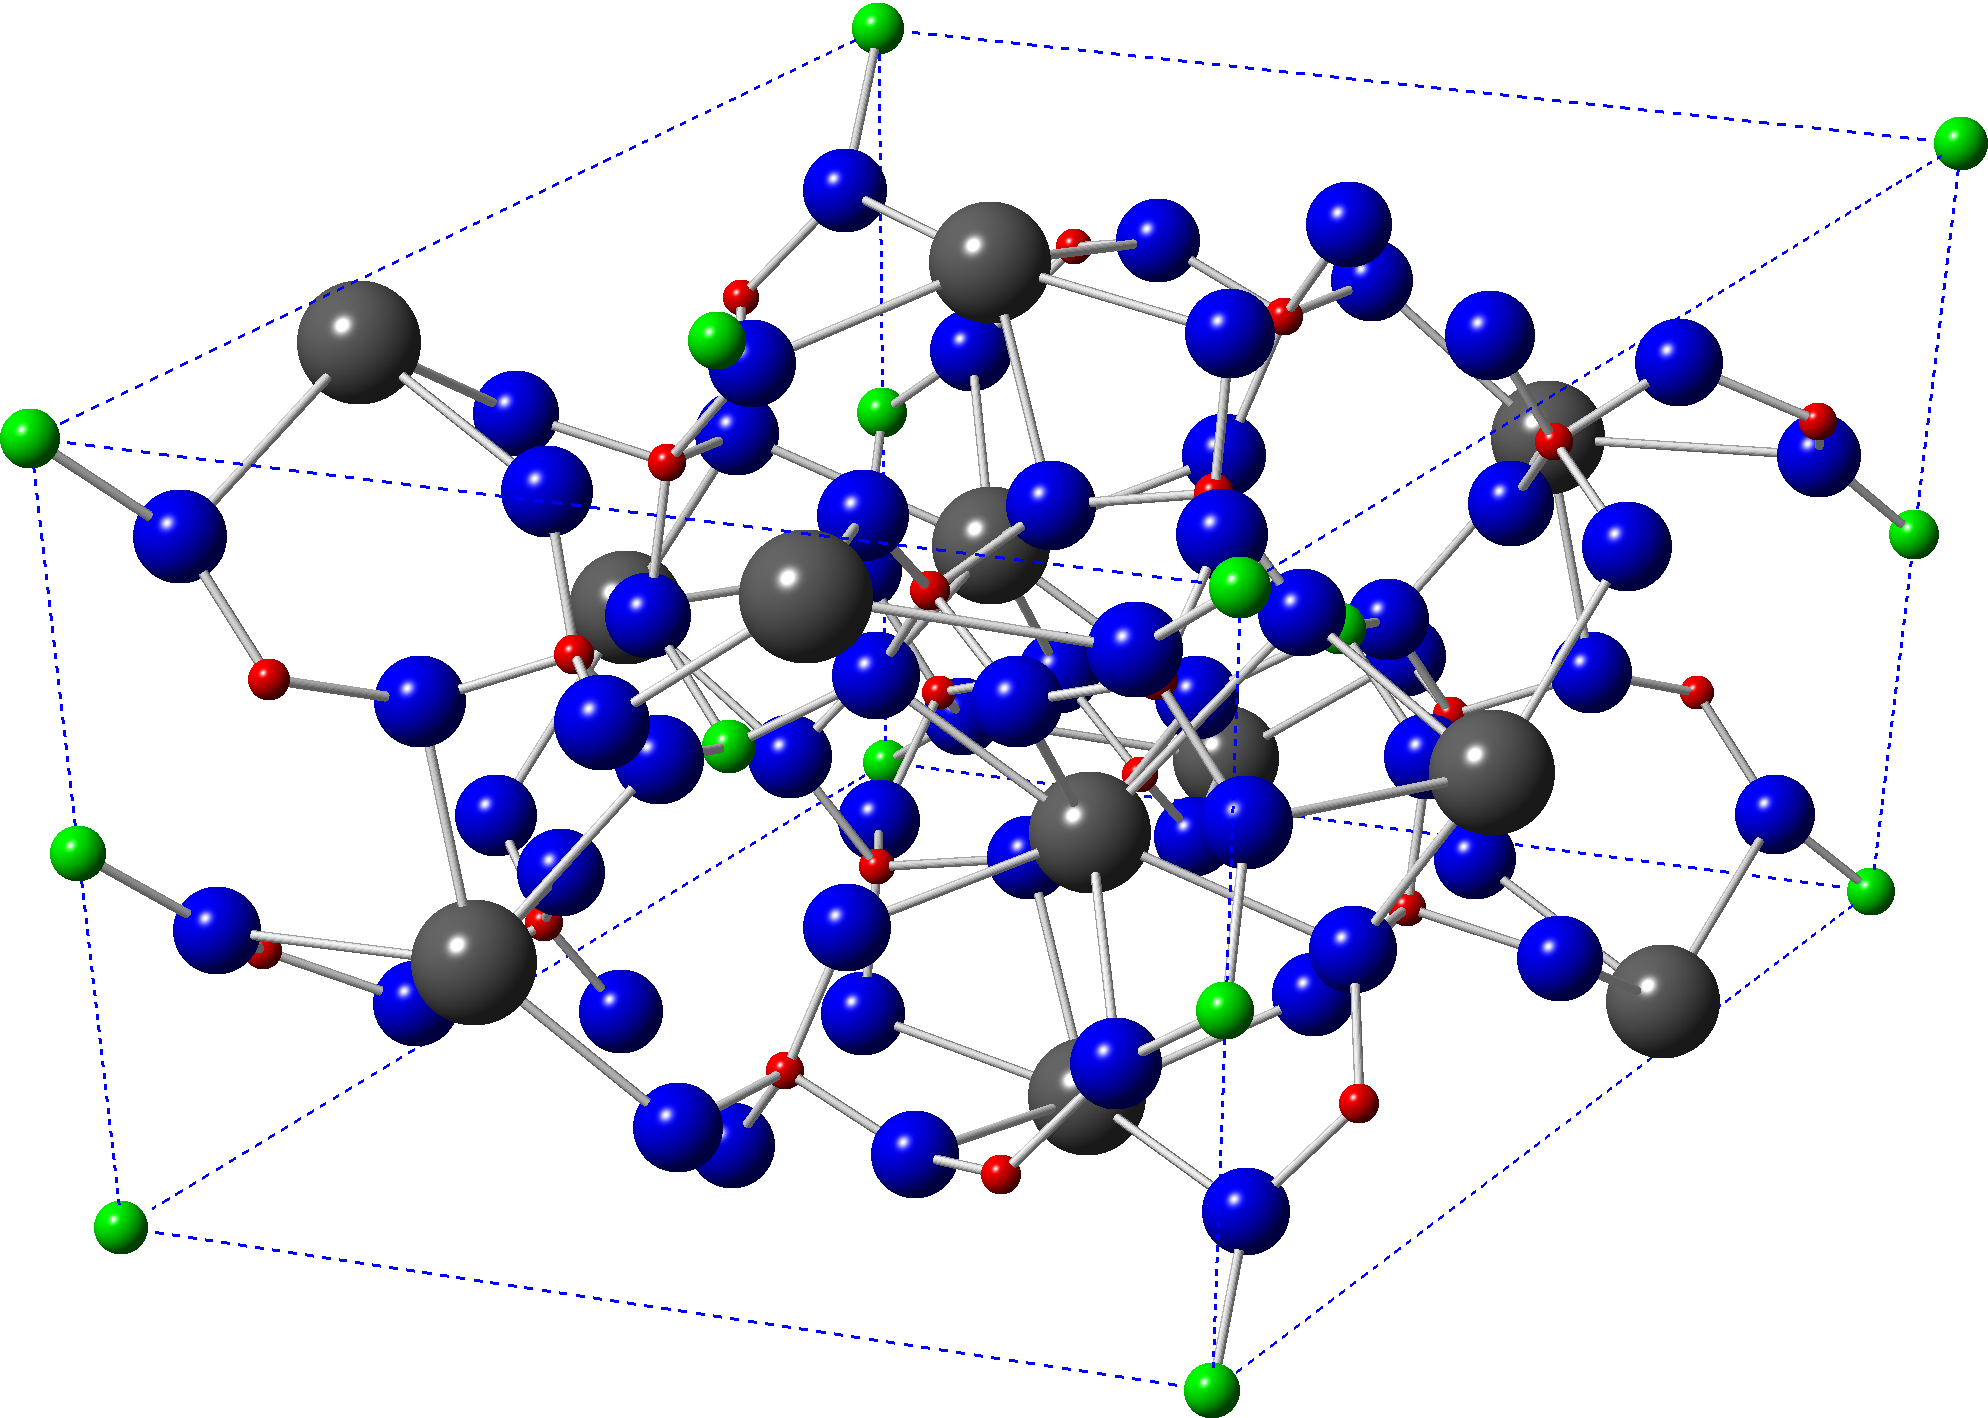
\includegraphics[height = 0.27\textwidth]{img/rgto-sol-1}
	}{\caption{%
		\texttt{0@g1,1@f1g1,2@b1d1,3@f1g4}\\(正确解)%
	}}
	\ffigbox[0.4\textwidth]{%
		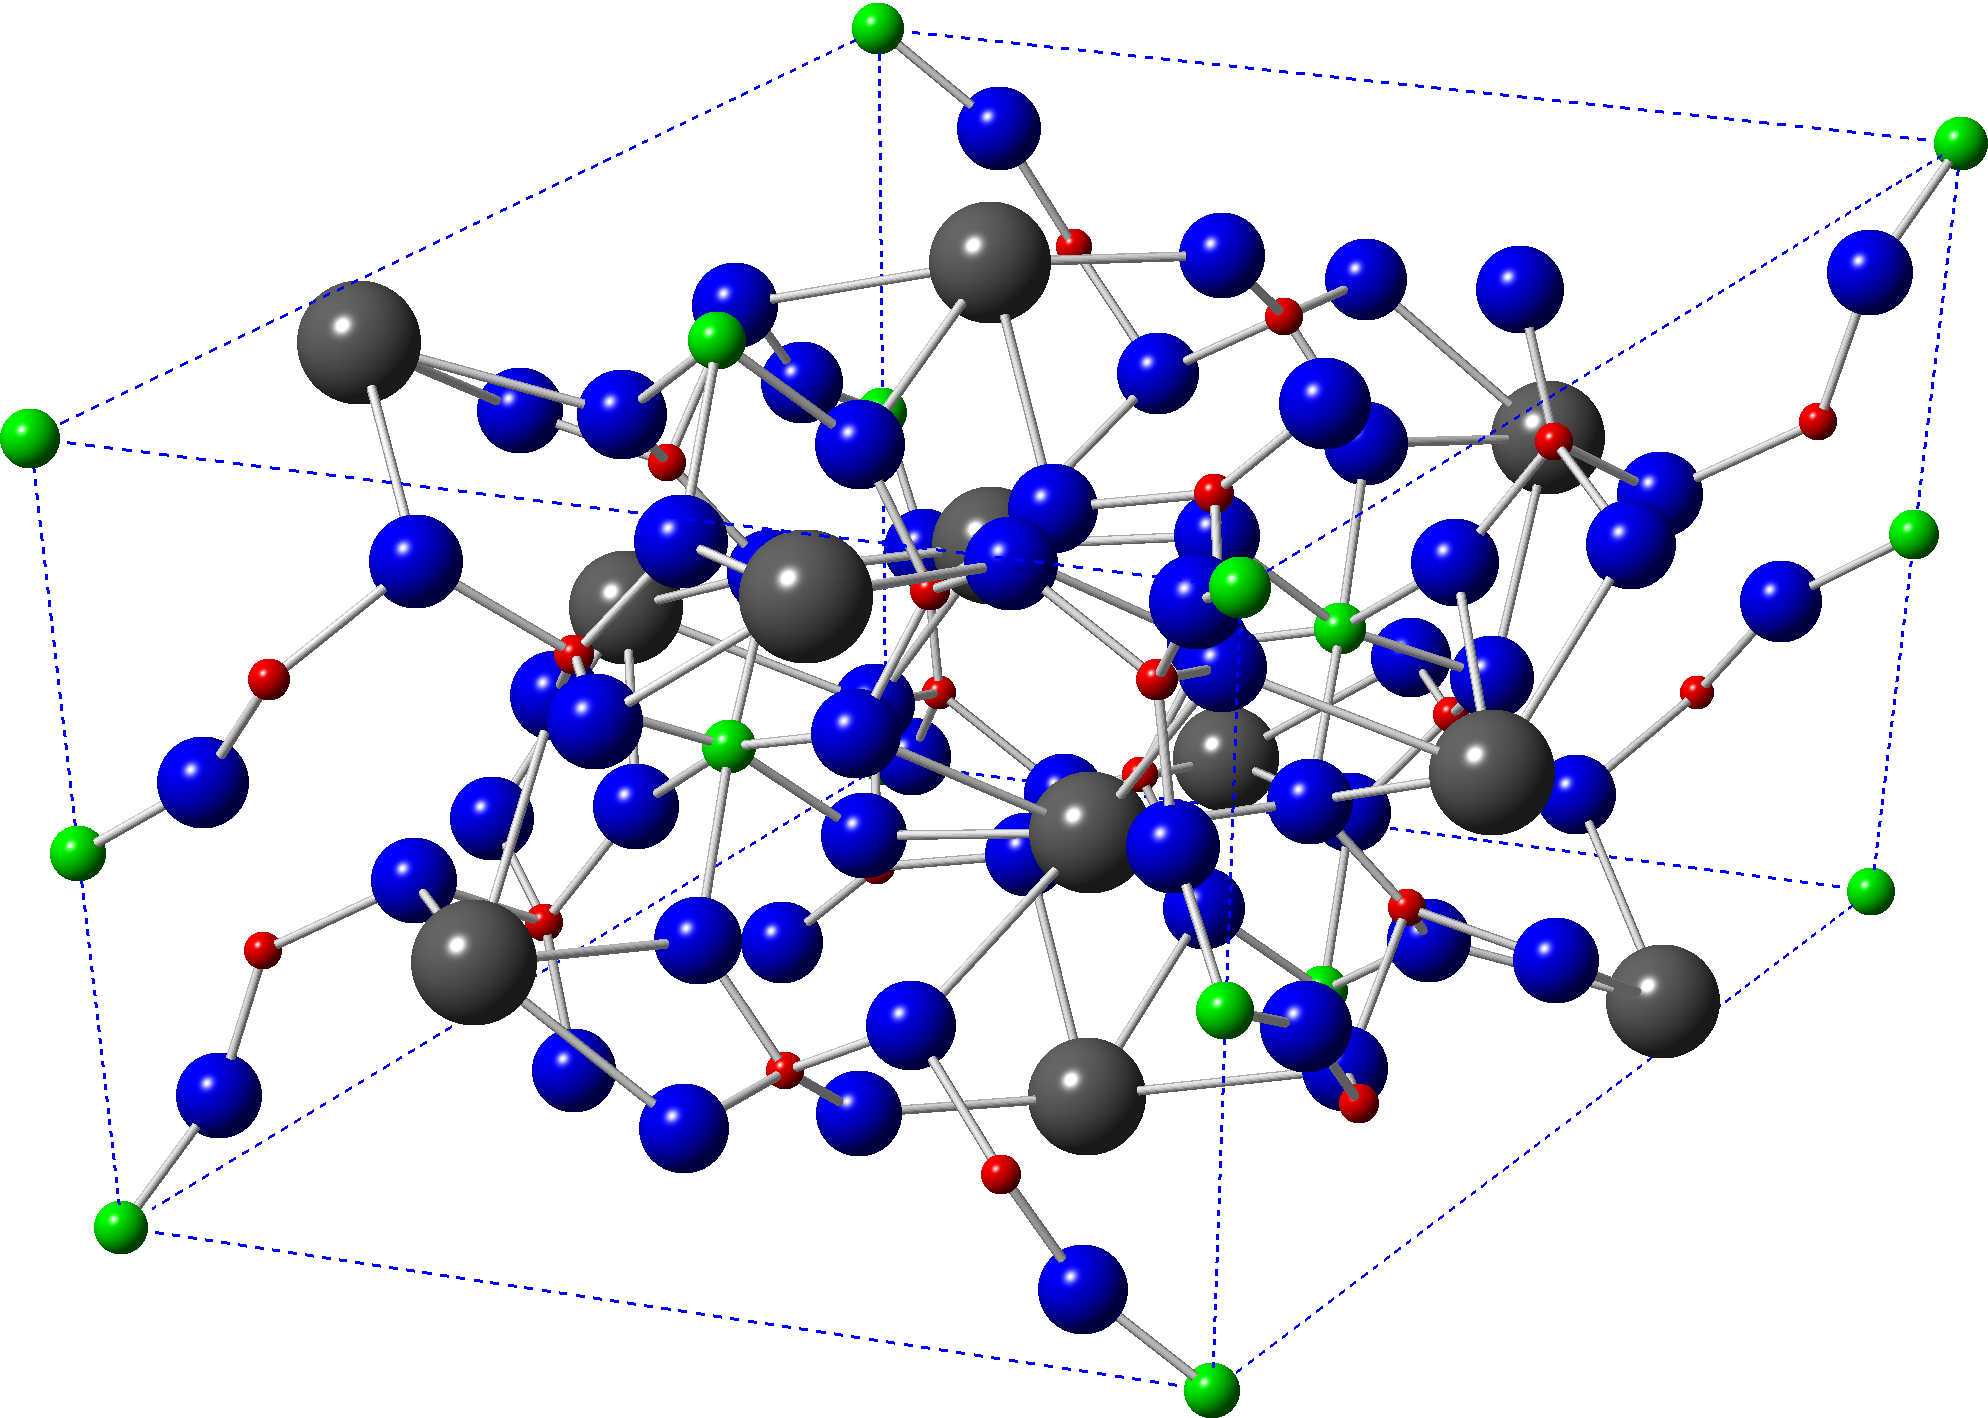
\includegraphics[height = 0.27\textwidth]{img/rgto-sol-2}%
	}{\caption{%
		\texttt{0@g1,1@f1g1,2@b1d1,3@f1g4}\\(\ce{Ge^{4+}} 配位多面体畸变严重)%
	}}
\end{subfloatrow}\\[0.4em]\begin{subfloatrow}
	\setlength{\columnsep}{1.5em}
	\ffigbox[0.4\textwidth]{%
		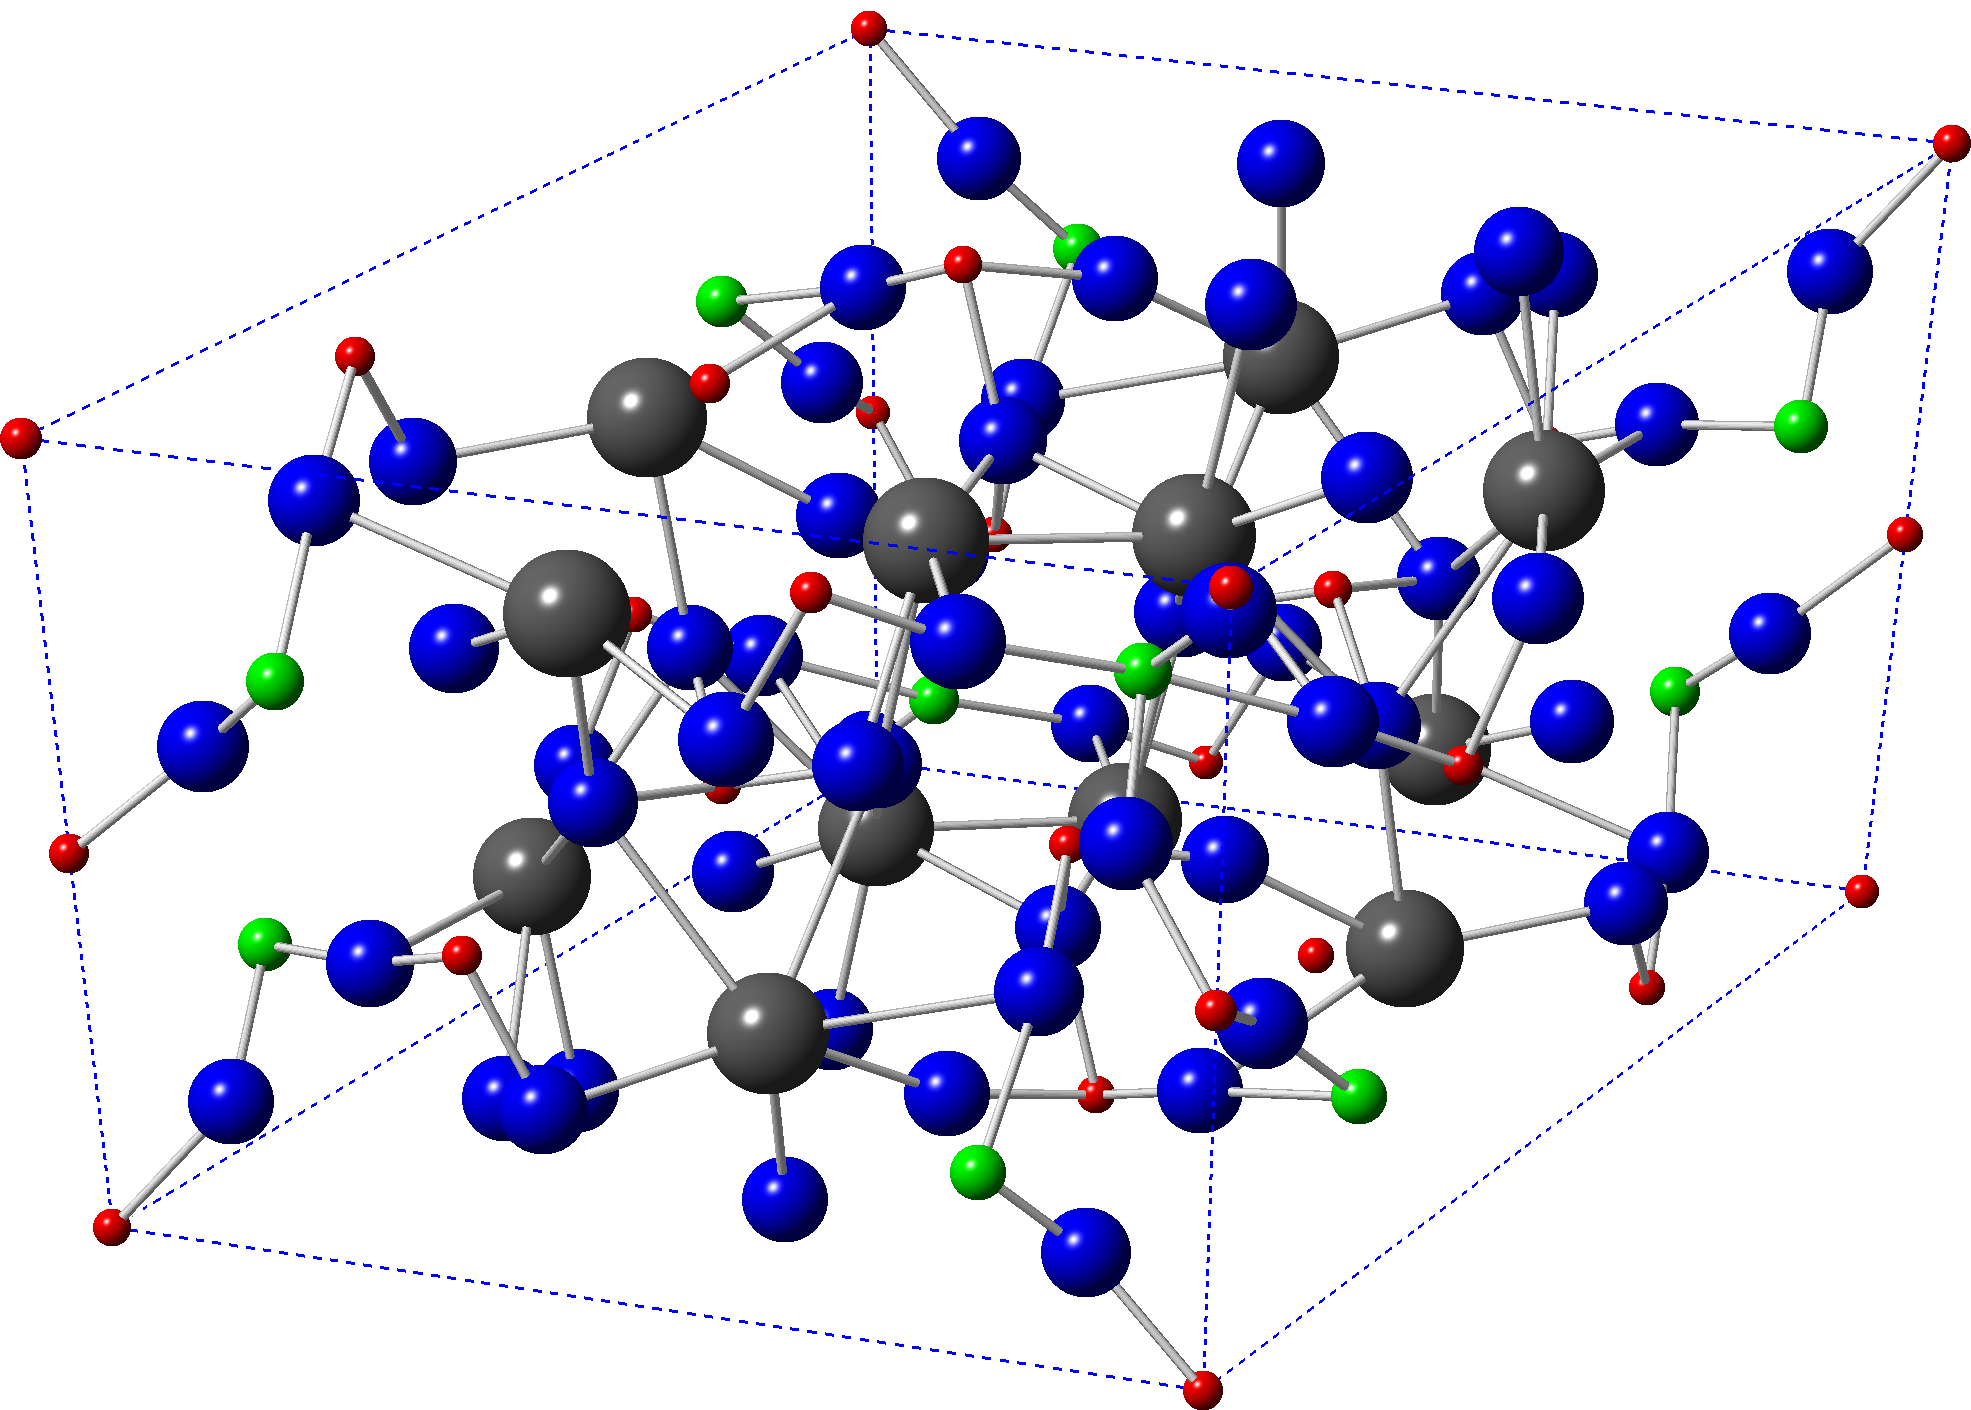
\includegraphics[height = 0.27\textwidth]{img/rgto-sol-3}%
	}{\caption{%
		\texttt{0@g1,1@b1d1g1,2@f1,3@f1g4}\\($b$ 位置的
		\ce{Ge^{4+}} 为 6 配位,\\其它位置的 \ce{Ge^{4+}} 为 3 配位)%
	}}
	\ffigbox[0.4\textwidth]{%
		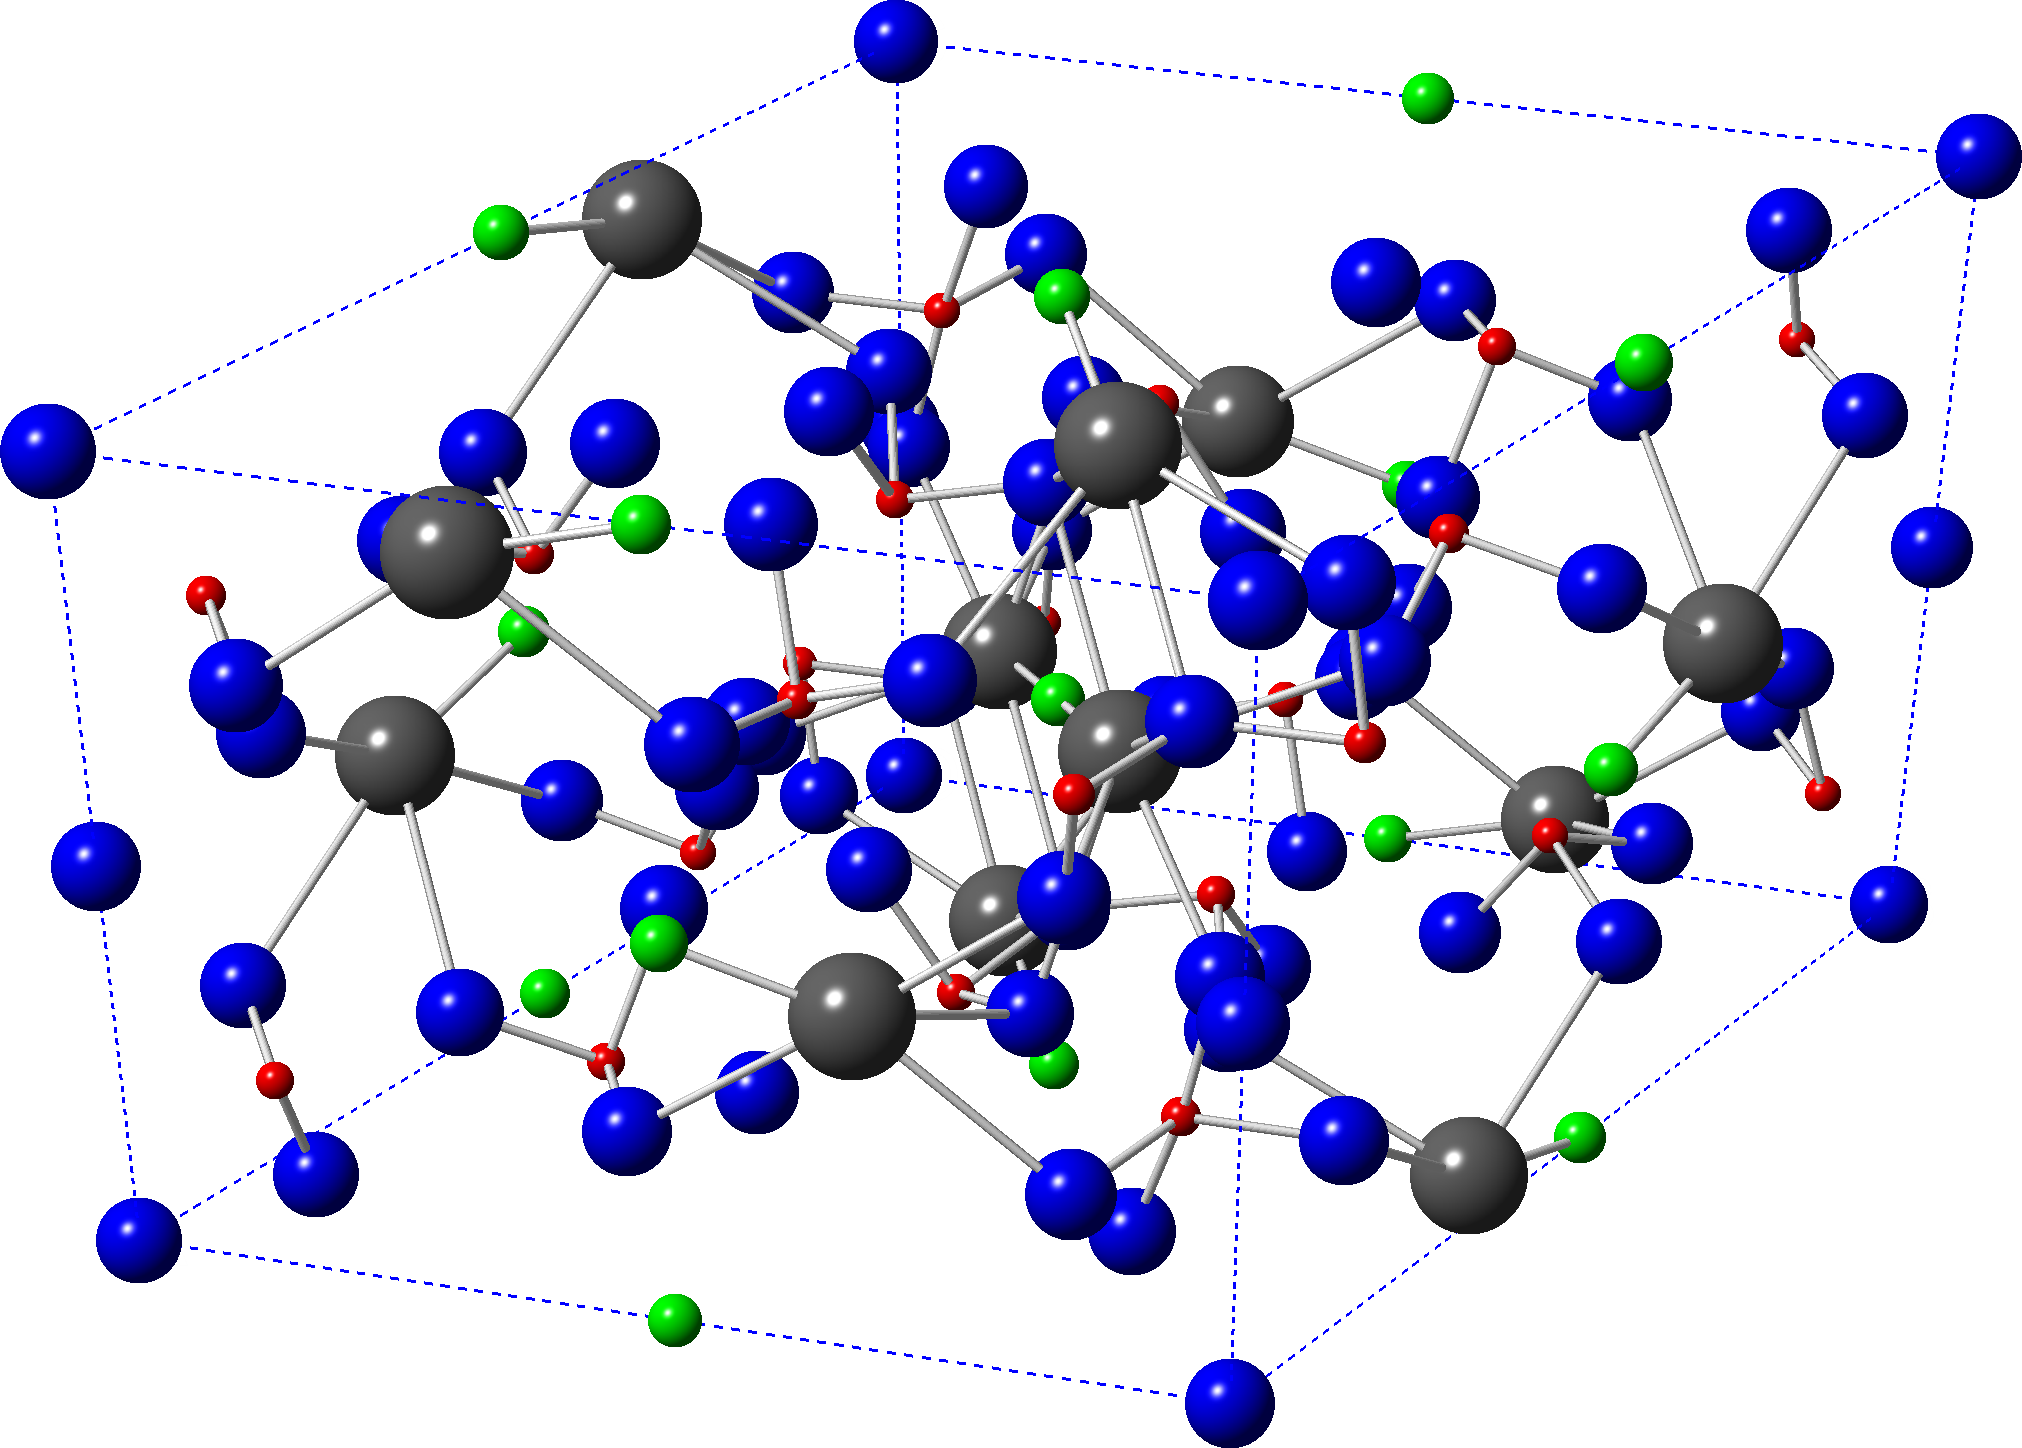
\includegraphics[height = 0.27\textwidth]{img/rgto-sol-4}%
	}{\caption{%
		\texttt{0@g1,1@f1g1,2@e1,3@b1d1f2g3}\\(在有孤立 \ce{O^{2-}}
		的前提下,\\每个 \ce{Ti^{4+}} 被 2 个 \ce{Rb+} 配位)%
	}}
\end{subfloatrow}}{\caption{“0009563”的一些解}\label{fig:9563-sol}}
\vspace{\slop{-0.6em}}
\end{figure}

\section{讨论和小结}
\subsection{关于动态剪枝的讨论}\label{ssec:prune-discus}

如第 \ref{ssec:incr-epc} 小节所述,Wyckoff 位置种类较多的空间群对于原子数稍多的
结构往往会生成极大量的可行 EPC;其内存溢出的潜在问题可以用增量生成 EPC 解决,
但其使结构测定的时间复杂度发生爆炸性增长仍是一个严重的问题。\textcite{lu1965}%
在求解 \ce{V2Ga5} 结构时筛选 EPC 的思路对我们有一定的启发:其根据对晶胞几何属性
的分析得出了各个 Wyckoff 位置之间的互斥关系。第 \ref{ssec:epc-discus} 小节指出,
可以通过在 \emph{decryst} 中引入涉及多于一个 Wyckoff 位置的占据数约束来应用
Wyckoff 位置的互斥关系;然而,这样的互斥关系在很多时候难以手工进行推导。

事实上,如果从深度优先树搜索的角度考虑,不难注意到生成 EPC 时的互斥约束也可以
放到剪枝的框架之下来理解:例如对于 \ce{V2Ga5},因为 $a$、$b$ 位置互斥,在其中
一个位置有占据时另一位置被占据的子树在搜索时就被剪掉了。在此背景之下,我们可以
沿用 \ref{ssec:epc-filter} 小节中利用原子重叠评估函数进行 EPC 筛选的思路,不再
手工推导互斥关系,而是动态地对互斥关系进行检测:在树搜索中时实时地对当前节点
所代表的(部分或全部原子的)EPC 进行针对原子重叠的统计分析或全局最优化,
并将不可能产生无碰撞晶体模型的子树剪掉。

如果要实现这样的动态剪枝,那么 EPC 的生成和(针对原子重叠而非衍射谱的)统计分析
或全局最优化将必须在同一步骤中进行,因此 \emph{decryst} 的设计和实现必须经过
大幅度的修改:在搜索过的每个节点上加入统计分析会明显增加树搜索的复杂度,
而全局最优化更是如此,因此动态剪枝必须是可选的,而且在启用动态剪枝时还必须
考虑树搜索的并行化问题,此外参数取值的遍历顺序(例如 $a_1b_1 \rightarrow
a_2b_1 \rightarrow \cdots \rightarrow a_1b_2 \rightarrow \cdots$ 和
$a_1b_1 \rightarrow a_1b_2 \rightarrow \cdots \rightarrow a_2b_1 \rightarrow
\cdots$)对算法复杂度的影响应该也是需要考虑的。不过有必要指出,在晶体学
软件中类似的情况不是只在 \emph{decryst} 里出现:例如为了将电荷反转法
(参考第 \ref{sec:reci-meth} 节)应用于衍射峰之间常有明显重叠的粉末
衍射数据,相应的算法\parencite{baerlocher2007}须要实时地对衍射峰的
划分方案进行调整,而分峰在倒空间法中原本通常是相对独立的步骤;
事实上,UACIEM\parencite{ma2004}就是一种动态分峰算法。

\subsection{其它讨论}

如第 \ref{ssec:epc-filter} 小节所述,除了在求解之后用于筛除发生原子重叠的解
模型以及在求解过程中实时排除发生重叠的晶体模型之外,本文中的原子重叠评估函数
也可以用于在求解前筛除不可能产生无重叠晶体模型的 EPC。更复杂的评估函数,例如
考虑键角、配位数、成键类型、原子链类型等等因素的那些\parencite{li2012},
从原则上看应该也可以用于类似用途,而且从实践上看肯定会有重要的意义:
例如要是能实际使用这样的评估函数,我们在求解“0000428”结构时就可以
很容易地拉开正确解和错误解在目标函数值上的差别,而在求解“0009563”
结构时也能极大地简化最后的手工(目视)筛选步骤。

从本章中大部分测试结构的求解过程可见,我们如果能自动化地实现对等价 EPC 和等价
晶体模型的检测,就能进一步提升结构测定的效率。前一问题大概可以通过按局部对称性
(site symmetry)对 Wyckoff 位置进行分组(例如 $R\bar3$ 空间群中 $d$、$e$
位置的局部对称性均为 $\bar1$),然后为对称操作可能导致的组内互变关系(例如
$R\bar3$ 空间群中 $(0, 0, 1/2)$ 平移可以使 $a/b$、$d/e$ 位置互变)
构造查找表的方式来处理。后一问题大概须要通过对某种特征性的指标进行
聚类分析来实现,而 \emph{CALYPSO}\parencite{wang2012}中的成键特征矩阵
(bond characterisation matrix)方法可能对这一指标的构造有一定的启发意义。

如第 \ref{ssec:epc-filter} 小节所述,即使在求解前筛除不可能产生无重叠晶体模型
的 EPC,并在求解中实时排除发生重叠的晶体模型,我们最后仍然可能得到发生重叠的解
模型;本人认为,发生这种现象的根本原因是某些 EPC 不能产生 $R$ 因子很小而且同时
不发生原子重叠的晶体模型,或者至少只能以很小的概率得到这样的模型。出于这一原因,
我们目前仍然须要在求解之后筛除发生重叠的解模型;另一种应该可行的思路是在目标函数
中以一种非线性的方式组合 $R$ 因子和原子重叠评估函数,从而使得目标函数值
在趋于零时被 $R$ 因子和评估函数值中较大的那个数值决定。

\subsection{本章小结}

\emph{decryst} 的设计追求简洁、灵活,而本人也希望其中的技巧可以在更多的晶体学
软件中得到应用。在现有自动化工具的配合下,用 \emph{decryst} 能简单地实现相当
复杂的求解流程:利用重原子法的求解,统计分析和全局最优化后基于 Bragg $R$
因子的等效点系组合(EPC)筛选,求解前筛除必发生原子重叠的 EPC、最优化中实时
排除存在原子重叠的晶体模型、求解后筛除仍发生原子重叠的 EPC,等等。为了演示
\emph{decryst} 的基本用法和常用技巧,本人从美国矿物学家晶体结构数据库(AMCSD)
中选取了若干个不同晶系和复杂度的测试结构,并成功地对它们进行了求解。

\begin{rquote}{0.1\textwidth}
	Almost anything in software can be implemented, sold, and even used, given
	enough determination.  There is nothing a mere scientist can say that will
	stand against the flood of a hundred million dollars.  But there is one
	quality that cannot be purchased in this way, and that is reliability.
	The price of reliability is the pursuit of the utmost simplicity.
	It is a price which the very rich find most hard to pay.
\end{rquote}
\rightline{--- C. A. R. Hoare (\cite*{hoare1981})}

% vim:ts=4:sw=4
